\documentclass[custom]{linearbook}
\usepackage{float}
\usepackage{xchoices}
\usepackage{extarrows}
\usepackage{arydshln}
\usepackage{physics}

\begin{document}
% \tikzexternaldisable

\frontmatter
\pagenumbering{Alph}
% 封面
%--------------------------------------------------------------------------
\bookmark[page=1, level=1]{封面}

\includepdf[noautoscale=true, width=\paperwidth]{images/cover.pdf}

% 扉页
%--------------------------------------------------------------------------
\pagenumbering{roman}
\setcounter{page}{1}
\pagestyle{front}
\clearsidenotenumber
\newgeometry{includemp=true,
             inner=2cm,outer=2cm,
             top=2cm,bottom=1.5cm,
             headsep=0.5cm,headheight=0.5cm,
             footskip=0.7cm,
             marginparsep=0cm,marginparwidth=0cm}
\thispagestyle{empty}
\bookmark[page=2, level=1]{扉页}

\begin{tikzpicture}[remember picture,overlay]
    \node at (current page.north west)
      {
        \begin{tikzpicture}[remember picture,overlay]
          \draw[fill=lbdeepblue,draw opacity=0]
            ++(0,-2cm) rectangle ++(\paperwidth,-4pt);
          \node[color=lbdeepblue,text width=13cm] (text)
            at  (0.5\paperwidth,-0.25\paperheight)
            {\titlefont\fontsize{40}{80}\selectfont  线性代数与解析几何\\[0.45cm] 入门讲义};
          \node[color=lbdeepgreen,below right,text width=13cm] (V) at ($(text.south west)+(0.5em,-1em)$)
          {\fontsize{13}{15}\selectfont \fontspec{Palatino-Roman} Linear Algebra and Analytic Geometry\\ Introductory Notes};
          \draw[line width=2pt,color=lbgreen]
            ++(2cm,-2cm) |- ($(text.south east)+(0,-2.5cm)$);
        \end{tikzpicture}
      };
\end{tikzpicture}

\vspace*{10cm}

\hspace{0.15\linewidth}\begin{minipage}{0.71\linewidth}
  % \zihao{5}
  \begin{flushright}\fontspec{Palatino-Roman}\selectfont\titlefont
    彭康书院学业辅导与发展中心志愿者部~~编写
\date{\zhtoday}  
\end{flushright}
\end{minipage}

\vfill

\begin{figure}[H]
	\centering
	\includegraphics[scale=0.1]{xdt-logo.png}
\end{figure}

\restoregeometry

% 版权页
%--------------------------------------------------------------------------
%\input{other/copyright.tex}

% 作者简介
%--------------------------------------------------------------------------
\chapter*{编写人员简介}
\addcontentsline{toc}{chapter}{编写\&排版人员简介}
\vspace{-3cm}

(按首拼字母排序)

\vspace{1em}

{\zihao{-2}\color{lbdeepblue}司秉钤}\quad 数试2101班学生,彭康学导团志愿者,在本份讲义中负责第二部分第2、3章编写。欢迎同学们来彭康学导团一起学习交流。同学们如有学习上的问题或者对本讲义有相关建议,请联系邮箱\url{2360804879@qq.com},希望和同学们一起学习进步。

\vspace{1em}

{\zihao{-2}\color{lbdeepblue}石学凯}\quad 智造钱2101班学生,彭康学导团成员,在本份讲义中负责第三部分第8、9章编写。希望和大家一起学习,无限进步。

\vspace{1em}

{\zihao{-2}\color{lbdeepblue}许祺}\quad 金禾2101班学生,彭康学导团热心志愿者,在本份讲义中负责第二部分第6章和第三部分第7章的编写。啥也不会,需要学习。对本讲义提出意见/勘误/合作请联系邮箱\url{2977038022@qq.com}。

\vspace{1em}
{\zihao{-2}\color{lbdeepblue}袁方}\quad 信息2105班学生,彭康学导团志愿者部成员,在本份讲义中负责第二部分第4、5章的编写。本人才疏学浅,所写不周之处还需要大家多多指正。最后希望大家认真学习,勤于思考,培养对数学学习的兴趣。

\vspace{1em}

{\zihao{-2}\color{lbdeepblue}袁思敏}\quad 大数据001班学生,在本份讲义中负责第一部分的编写,邮箱\url{1653867189@qq.com}。

\vspace{1em}

{\zihao{-2}\color{lbdeepblue}张恺}\quad 核工A002班学生,彭康学导团志愿者部部长,乐于分享,偏爱\LaTeX 排版,在本份讲义中负责全书的排版。自2021年加入彭康学导团大家庭以来,负责多份资料的编写和排版任务,包括高数等课程的真题集、《大学物理笔记(上、下)》、《流体力学·复习要点》等。

\vspace{2em}

在此,对以上牺牲个人宝贵时间来完成这份讲义的同学表示衷心感谢!

% 序
%--------------------------------------------------------------------------
%\input{other/forword.tex}

% 前言
%--------------------------------------------------------------------------
\chapter*{前言}
\addcontentsline{toc}{chapter}{前言}

\plainsection*{献给读者}

西安交通大学的学弟学妹们: 你们好!

\subsubsection*{你为何收到这份讲义}
秋风生渭水,落叶满长安,欢迎你们来到古都西安。在飒爽的季节里见到你们,我们的记忆里常常涌起初到交大时的激动与迷茫。各个社团与活动与学业压力一同到来,每个人都在尝试着平衡学习与生活——这是大学生活天平的两端。交大是古城西安中文化底蕴最深厚,最务实的学校之一,而作为交大学子的你们在大一面对的最重要的科目之一就是线性代数,在未来的许多专业课程中,线性代数和高等数学的基础知识都会发挥非常重要的作用。\textbf{彭康学业辅导与发展中心(彭康学导团)}特定准备了一份高等数学引导讲义,带你理解高数学习的要领。另外,欢迎没有加入QQ群\textbf{彭小帮2.0(397499749)}的同学前来交流学习,这是交大进行学习交流的基地之一,有众多同辈同学与前辈的学长学姐与你共同学习。

\subsubsection*{你应该如何理解这份讲义}
这份讲义并不是严格标准的教学用书,只是一份引导性质的讲义。这份讲义\textbf{不可以替代上课听讲},但是可以帮助你课前预习与课后巩固。这份讲义是学长学姐的感悟与体验,但是你需要整理属于你自己的学习心得。\textbf{这份讲义的版权属于西安交通大学彭康学业辅导与发展中心,不可售卖,不可复印出售。}

\subsubsection*{当你学数学的时候,你在学习什么}
学习数学的时候,我们通常有两套语言在彼此交互:\textbf{纸面上的数学语言与脑海中的自然语言}。而许多同学没有学习好数学的根本原因,是困扰于数学语言而不知道某知识点的自然语言如何表述,这就导致在学习的过程中出现了困顿与阻滞的状态。因此,这份讲义\textbf{花开两朵,各表一枝},既注重数学知识与公式的引导,也强调使用自然语言说明清楚某个知识点的内涵与应用。

\subsubsection{本讲义的编写与阅读原则}

本讲义的编写按照《线性代数与解析几何》课本的顺序,上下梳理三部分知识点,注重知识点的连续与衍生应用。\textbf{轻推导,重实践},秉持“让交大每位学生顺利走入线代殿堂”的原则,左右横揽重点知识点与相关衍生习题。对于每一节的内容,\textbf{第一部分是知识点概览},会提纲挈领的告诉你学习这一节你需要掌握的内容与重点。\textbf{第二部分是知识点的背景叙述},帮助你复习预备知识,使各知识点彼此贯通。\textbf{第三部分会讲述具体知识点},会按照自然语言引导+数学语言结论的方式讲述知识点,是每一节的重中之重。\textbf{第四部分放在最后,是相关结论、二级思维、套路与习题结构的整合之处}。

\subsubsection{结束语}
怕什么真理无穷,进一步有进一步的欢喜。欢迎各位同学加入彭康学业辅导与发展中心,彭康书院的东19-114室是我们的线下大本营,里面有专门答疑的志愿者为你们答疑。此外,线上学习研究中心的基地是QQ群:彭小帮2.0(397499749),欢迎各位同学加入,我们永远欣喜于你们的到来。

\plainsection*{笔误及疏漏}

由于水平有限,编写组成员对本书中可能出现的错误深表歉意,并希望读者予以批评指正。

\vspace{3em}
\hfill\begin{minipage}{7cm}
	\begin{flushright}\kaiti
		彭康书院学业辅导与发展中心·志愿者部\\
		\zhtoday
	\end{flushright}
\end{minipage}

% 致谢
%--------------------------------------------------------------------------
%\input{other/acknowledgment.tex}

% 重排按
%--------------------------------------------------------------------------
%\input{other/retypestate.tex}

% 目录
%--------------------------------------------------------------------------
\newpage
\bookmark[page=16, level=0]{目录}
\newgeometry{includemp=true,
    inner=2cm,outer=1.2cm,
    top=2cm,bottom=1.5cm,
    headsep=0.5cm,headheight=0.5cm,
    footskip=0.7cm,
    marginparsep=0.4cm,marginparwidth=3cm}
\pagestyle{toc}
% \addtocontents{toc}{~\kern-10em{\color{lbgreen}\hrule width \textwidth height 2pt depth 0pt}} % 目录添加横线
\tableofcontents
\restoregeometry
\cleardoublepage                % 必须加上否则,会出错

\mainmatter
\pagestyle{main}
%---------------------------------------------------------------------------
% Chapters
%---------------------------------------------------------------------------
% \chapter{占位章}
% \makeatletter
\renewcommand{\@makeschapterhead}[1]{%
  \addtocontents{toc}{\protect\hypertarget{chap:\thechapter}{}}%  跳转回目录
  \checkoddpage
  \@ifoddpage{ % 奇数页
      \begin{tikzpicture}[remember picture,overlay]
        \node at (current page.north west)
          {
            \begin{tikzpicture}[remember picture,overlay]
              \draw[fill=lbdeepblue,draw opacity=0]
                ++(0,-2cm) rectangle ++(\paperwidth,-4pt);
              \node[inner sep=12pt,below left] (chapter)
                at  +(\paperwidth-1.2cm,-2.2cm) {\color{lbdeepblue}\titlefont\Huge
                \texorpdfstring{\protect\hyperlink{chap:\thechapter}{#1}}{#1}};
              \draw[line width=2pt,color=lbgreen] 
                ++(\paperwidth-1.2cm,0) |- ($(chapter.south west)+(0,4pt)$);
            \end{tikzpicture}
          };
      \end{tikzpicture}
      \vspace{7cm}
    % 页眉
    % \renewcommand{\chaptermark}[1]{\markboth{\kaiti #1}{}}%
    \renewcommand{\chaptermark}[1]{\markboth{\normalfont\kaiti %
    \protect\hyperlink{chap:\thechapter}{#1}  %
    }%
    {}%
    }%
    \chaptermark{#1}%
  }{% 偶数页
      \begin{tikzpicture}[remember picture,overlay]
        \node at (current page.north west)
          {
            \begin{tikzpicture}[remember picture,overlay]
              \draw[fill=lbdeepblue,draw opacity=0]
                ++(0,-2cm) rectangle ++(\paperwidth,-4pt);
              \node[inner sep=12pt,below right] (chapter)
                at  +(1.2cm,-2.2cm) {\color{lbdeepblue}\titlefont\Huge
                \texorpdfstring{\protect\hyperlink{chap:\thechapter}{#1}}{#1}};
              \draw[line width=2pt,color=lbgreen] 
                ++(1.2cm,0) |- ($(chapter.south east)+(0,4pt)$);
            \end{tikzpicture}
          };
      \end{tikzpicture}
      \vspace{7cm}
    % 页眉
    % \renewcommand{\chaptermark}[1]{\markboth{\kaiti #1}{}}%
    \renewcommand{\chaptermark}[1]{\markboth{\normalfont\kaiti %
    \protect\hyperlink{chap:\thechapter}{#1}  %
    }%
    {}%
    }%
    \chaptermark{#1}%
  }%

  % 上面这个空行不能删掉
}
\makeatother

\chapter*{绪论}
\addcontentsline{toc}{chapter}{绪论}

众所周知,雷达是一个信息传输和处理的系统,它区别于通讯系统之处,在于信息的调制过程发生在目标散射之时.显然,雷达信息传输过程也会受到各种外界(自然和人为的)干扰和内部噪声干扰.所以雷达信号理论的发展也是建立在信息论,特别是信号检测理论的基础之上的.

早在1943年North\mn{重排版删去了原著的音译名.}\refcite{1} 提出匹配滤波器理论,大大推动了雷达检测能力的提高. 1950年Lawson把匹配滤波器理论系统地载入著名的专著\refcite{2}.

1950年Woodward\refcite{3} 把香农(Shannon)所建立的基础信息论\on{Коrельникоn也是基础信息论的创始人之一.}中关于信息量的概念推广应用于雷达信号检测中来,认为从提取最多有用信息的观点出发,理想的雷达接收机同样应该是一个后验概率的计算装置.

从统计学的观点看,雷达观测是一个典型的统计判断过程. Hance\refcite{4} 和Marcum\refcite{5} 最早把Middleton \refcite{6} 和Neyman\refcite{7} 建立的统计检测理论应用于雷达. Swerling\refcite{8} 结合雷达目标起伏特性建立了四种目标起伏模型,得到许多有用的目标检测数据.

在信号检测理论的历史上,曾出现过许多最佳准则,已经证明,从各种最佳检测准则出发,导出的最佳信号检测系统都是由一个似然比计算装置和一个门限检测器组成的.根据不同的最佳准则,门限取值不同.在高斯噪声下对确知信号的似然比计算装置实质上就是一个匹配滤波器.至此,按最大信噪比准则导出的匹配滤波器与按统计判决理论导出的似然比计算装置之间的内在联系便显而易见了.

为了解决杂波中的信号检测问题, Urkowitz\refcite{9} 把匹配滤波器理论推广到色噪声的场合,提出``白化滤波器''和''逆滤波器''的概念.之后, Manasse\refcite{10} 研究了同时存在白噪声和杂波干扰下的最佳滤波器,为抑制杂波波形优化问题打下了理论基础.

Cramer\refcite{11} 继承Fisher 的工作,建立了经典的参量估计理论. Slepian 把经典的最大似然估计理论应用于雷达\refcite{12},稍后SkoInik\refcite{13} 对雷达测量的理论精度作了系统的分析和总结.

值得指出的是伍德沃德不仅在发展雷达倍号检测理论上作出了很大贡献,而且在著名的著作\refcite{14} 中提出有名的雷达模糊原理,定义了模糊函数及分辨常数等新概念,奠定了雷达分辨理论的基础.并首次触及波形设计问题,指出距离分辨力和测量精度取决于信号的带宽而非时宽,从而大大推动了雷达信号理论的发展.稍后的Helstrom的著作\refcite{15} 应该说也是雷达信号统计检测理论方面很好的一本参考书.

二次世界大战期间及战后初期,在实现了雷达信号最优处理的前提下,典型的脉冲雷达在同时提高发现能力、距离和速度测量精度以及分辨力方面遇到了不可克服的矛盾,为了解决这个问题,也为了反雷达侦察的需要,各国先后开展了应用``复杂波形''代替传统的脉冲信号的研究.最早获得实际应用的是线性调频脉冲压缩信号\mrefcite{16}{22}.以后相继出现非线性调频、相位编码\refcite{23} 和相参脉冲串等大时宽--带宽信号.

由于雷达发射波形不仅决定了信号处理方法,而且直接影响系统的分辨力、测量精度以及抑制杂波能力等潜在性能.于是,波形设计就成了雷达系统最佳综合的重要内容,逐渐形成现代雷达理论的重要分支.

开始,人们希望找到一种``理想''的波形,以适应各种不同的目标环境和工作要求,很快就发现这种努力是徒劳的.

雷达波形设计一直沿着两种不同的途径进行研究,一种是Sussman等人\mrefcite{24}{26} 所走的波形综合的道路,通过模糊函数最优综合的方法,得到所需要的最优波形.遗憾的是这方面不仅遇到了数学上的困难,而且综合得到的复杂调制波形,也往往是技术上难以实现的信号.不过一维模糊函数的综合借助于相位逗留原理获得了较好的解决\refcite{27}. Rihaczek\refcite{28} 提出另外一种``简便的波形选择途径'',即根据目标环境图和信号模糊图匹配的原则,选择合适的信号类型.进而兼顾技术实现的难易程度,选择合适的信号形式和波形参数.近代先进的数字化多功能雷达大多采用多种发射信号,以适应不同的战术用途.随着电子战的发展,现代雷达面临的目标环境不仅复杂多端,而且是瞬息万变的,所以波形自适应是个值得重视的发展方向.

综上所述,可以看到,雷达信号理论的形成与发展,目的在于提高雷达信号传输的可靠性和有效性.显然,这里不是针对系统的某个环节或某个电路的具体措施,而是对整个系统进行最优综合.概括地说,雷达信号理论研究的课题包括从理论上探讨信号最优处理方法和最优波形的选择等两方面.这里涉及如何建立系统的数学模型,确定最优准则以及寻求最优系统结构(数学运算结构)等方面的问题.所以雷达信号理论是发展各种雷达新体制的理论基础.此外,雷达信号理论也是对实际雷达系统进行性能分析的理论指导,用以阐明实际雷达系统的合理性及改进的可能性.相信随着雷达信号理论的发展,雷达系统的威力、精度、分辨力以及反侦察、抗干扰能力必将得到进一步提高,雷达回波信号中所包含的有用信息必将得到更充分的利用.

雷达信号理论既然是设计近代雷达的理论基础,在培养高等科技人材的院校设置这门课程就显得十分必要了.当然,雷达信号理论涉及面很广,内容十分丰富,本书只是个导论性的书籍,着重介绍雷达信号最优检测、最优估计、分辨理论以及波形设计等基本问题,为读者进一步掌握近代雷达理论提供必要的基础.

\plainsection{参考文献}

\begin{references}
    \refitem \mn*{原著年代久远,参考文献格式不尽规范,但囿于重排者时间和精力有限,暂保留原著样式,只做微调.}D.O.North,Analysis of Factors which Determine Signal-to-noise Discrimination in Pulsed Carrier Systems, RCA Rept, PTR-6C, June 1943. (PIEEE Vol 51, pp 1015, 1969重印).
    \refitem J. L. Lawson and G. E. Uhienbeck, Threshold Signals, Radiation Lab. Series NO.24, McGraw-Hill, 1950.
    \refitem P. M. Woodward and I. L. Devies, A Theory of Radar Information, Phil. Mag. Vol 41, pp 1001--1017, 1950.
    \refitem H. V. Hance, The Optimization and Analysis of Systems for the Detection of Pulsed Signals in Random Noise, D. Sc Dissertation, MIT Cambridge Mass, 1951.
    \refitem J. I. Marcum, A statistical Theory of Target Detection by Pulsed Radar, RAND Corp Mem.RM-754, Dec.1947; RM-753, July 1948. (IRE Trans, Vol IT-6 NO.2, 1960重印).
    \refitem D. Middleton and J. H. Van Vleck, Theoretical Comparison of the Visual, Aural and Meter Reception of Pulsed Signals in the Presence of Noise, J. of Appl. Phys. Vol 17, pp 940--971, Nov. 1946.
    \refitem J. Neyman and E. J. Pearson, On the Problem of the Most Efficient Tests of Statistical Hypothesses, Philos. Trans. Royal Soc. London Series A, 23 pp 289--337, 1931.
    \refitem P. Swerling, Probability of Detection for Fluctuating Targets RAND Corp Res Mem. RM-1217 March 1954.(IRE Trans, Vol IT-6, pp 269--308 April 1960重印).
    \refitem H. Urkowitz, Filter for Detection of Small Signals in Clutter, J. Appl. Phy. Vol 24 pp 1024, July 1953.
    \refitem R. Manasse, The Use of Pulse Coding to Discriminate Against Clutter, AD260. 230, 1961.
    \refitem H. Cramer, Methods of Mathematical Statistics, Princeton University Press, 1946.
    \refitem D. Slepien, Estimation of Signal Parameters in the Presence of Noise, IRE Trans. Vol IT-4, pp 68--89. March 1954.
    \refitem M. I. Skolnik, Theoretical Accuracy of Radar Measurements PGANE Trans. ANE-7 NO.4 pp 123--129, 1960.
    \refitem P. M. Woodward, Probability and Information Theory with Application to Radar, McGraw-Hill, 1953.
    \refitem C. W. Helstrom, Statistical Theory of Signal Detection, Pergamon Press, 1960.
    \refitem E. Huffman, German Patent NO.768, 068, 1940.
    \refitem D. O. Sproule and A. J. Hughes, British Patent NO.604, 429, 1948.
    \refitem W. Cauer, German Patent NO.892, 772, 1950.
    \refitem R. H. Dicke, U.S. Patent, NO.2, 624, 876, 1953.
    \refitem S. Darlington, U. S. Patent, NO.2, 678, 997, 1954.
    \refitem Я. Д. Шнрман,Способ повышения разрешающей способности радиолока\-ционных станций и устройство для его осуществления, Авт. свид. NO.14\-6803 по Заявке NO.461974/40 от 25 Июля 1956.
    \refitem J. E. Chin and C. E. Cook, The Mathematics of Pulse Compression, Sperry Eng. Review Vol 12, pp 11--16 Oct. 1959.
    \refitem W. M. Sibert, A Radar Detection Philocophy, IRE Trans Vol IT-2, pp 204--221, Sept. 1956.
    \refitem C. H. Wilcox, The Synthesis Problen for Radar Ambiguity Function, AD 2394\-27, 1960.
    \refitem S. M. Sussman, Least-square Synthesis of Radar Ambiguity Functions, IRE Trans. Vol IT-8 NO.3 1962.
    \refitem J. D. Walf, G. M. Lee and C. E. Suyo, Radar Waveform Synthesis by Mean-square Optimization Techniques, IEEE Trans. Vol AES-5, July 1969.
    \refitem E. L. Key, E. N. Fowle and R. D. Haggarty, A Method of Designing Signals of Large Time-ba-ndwidth Production, IRE Int. Conv. Record pt 4 pp 146--155, 1961.
    \refitem A. W. Rihaczek, Radar Waveform Selection-A Simplified Approach, IEEE Trans. Vol AES-7, Nov. 1971.
\end{references}

% \chapter{占位章}
\cleardoublepage
\newgeometry{top=2.0cm,bottom=2cm,inner=2cm,outer=2cm}
\part{行列式}
\cleardoublepage
\restoregeometry

\chapter{行列式}

行列式对于刚上大学的我们而言是一个全新的概念,但掌握行列式并不难,最重要的部分是行列式的计算,学习计算套路并做题巩固就能熟练解题。

学习本章的要求如下:

\begin{enumerate}
    \item 领会行列式的定义;
    \item 学会使用对角线法则计算2阶和3阶行列式;
    \item 代数余子式的定义和性质;
    \item 行列式按行(列)展开;
    \item 正确使用行列式的有关性质化简、计算行列式;
    \item 掌握使用Cramer法则判定线性方程组解的存在性、唯一性及求出方程组的解。
\end{enumerate}

\section{行列式的定义与性质}

\subsection{引入——二阶行列式与一类二元线性方程组的解}

在初等数学中,我们用代入消元法求解二元和三元线性方程组,可以看出,线性方程组的解完全由未知量的系数和常数项所确定。

为了更清楚地表达线性方程组解与未知量地系数和常数项地关系,我们在本章先引入二阶行列式的概念,并在二阶行列式的基础上,给出$n$阶行列式的定义并讨论其性质,进而把$n$阶行列式应用于$n$元线性方程组。

行列式是一种常用的数学工具,在数学及其它学科中都有着广泛的应用。

\begin{example}
    用消元法解二元线性方程组

    \begin{equation}
        \left\{
        \begin{array}{c}
            a_{11}x_1+a_{12}x_2=b_1 \\
            a_{21}x_1+a_{22}x_2=b_2
        \end{array}
        \right.\label{eq1.1}
    \end{equation}
\end{example}

\begin{solution}
    用加减消元法可得

    \begin{equation}
        \left\{
        \begin{array}{c}
            (a_{11}a_{22}-a_{12}a_{21})x_1=b_1a_{22}-a_{12}b_{2} \\
            (a_{11}a_{22}-a_{12}a_{21})x_2=a_{11}b_{2}-b_{1}a_{21}
        \end{array}
        \right.\label{eq1.2}
    \end{equation}

    当$a_{11}a_{22}-a_{12}a_{21}\ne  0$时,求得方程组的解为

    \begin{equation}
        \left\{
        \begin{array}{c}
            x_1=\frac{b_1a_{22}-a_{12}b_{2}}{a_{11}a_{22}-a_{12}a_{21}} \\
            x_2=\frac{a_{11}b_{2}-b_{1}a_{21}}{a_{11}a_{22}-a_{12}a_{21}}
        \end{array}
        \right.
    \end{equation}
\end{solution}

为了记忆该公式,引入记号

$$\left|\begin{array}{ccc}
        a_{11} & a_{12} \\
        a_{21} & a_{22}
    \end{array}\right| \xlongequal{\rm def} a_{11}a_{22}-a_{12}a_{21} $$

并称之为\textbf{二阶行列式},其中$a_{ij}$称为行列式的\textbf{元素},$a_{ij}$的两个下标表示该元素在行列式中的位置,第一个下标称为\textbf{行标},表示该元素所在的行,第二个下标称为\textbf{列标},表示该元素所在的列,常称$a_{ij}$为行列式的\textbf{$(i,j)$元素}或\textbf{元}。

由二阶行列式的定义,\ref{eq1.2}式中$x_1$,$x_2$ 的分子也可以写成二阶行列式,即

$$
    b_1a_{22}-a_{12}b_{2}= \left|\begin{array}{ccc}
        b_1 & a_{12} \\
        b_2 & a_{22}
    \end{array}\right| , a_{11}b_{2}-b_{1}a_{21}= \left|\begin{array}{ccc}
        a_{11} & b_1 \\
        a_{21} & b_2
    \end{array}\right|  \\
$$

若记$D= \left|\begin{array}{ccc}
        a_{11} & a_{12} \\
        a_{21} & a_{22}
    \end{array}\right| , D_1=\left|\begin{array}{ccc}
        b_1 & a_{12} \\
        b_2 & a_{22}
    \end{array}\right| ,D_2= \left|\begin{array}{ccc}
        a_{11} & b_1 \\
        a_{21} & b_2
    \end{array}\right|  $,

则当$D \ne 0 $时,方程组\ref{eq1.1}有唯一解\mn{$D$称为系数行列式,$D_{j}$是用常数项 $b_{1},b_{2}$替换$D$中的第 $j$列($j=1,2$)。}
$$
    x_1=\frac{D_1}{D},x_2=\frac{D_2}{D}
$$

\begin{example}
    计算二阶行列式
    $\left|\begin{array}{ccc}
            5 & -1 \\
            3 & 2
        \end{array}\right| $
\end{example}

\begin{solution}
    $\left|\begin{array}{ccc}
            5 & -1 \\
            3 & 2
        \end{array}\right| =5\times 2-(-1)\times 3=13$
\end{solution}

\begin{example}
    解二元线性方程组
    $
        \left\{
        \begin{array}{c}
            3x_1-2x_2=1 \\
            2x_1+x_2=3
        \end{array}
        \right.
    $
\end{example}

\begin{solution}
    因为$ D=\left|\begin{array}{ccc}
            3 & -2 \\
            2 & 1
        \end{array}\right| =7\ne 0 $,且$D_1=\left|\begin{array}{ccc}
            1 & -2 \\
            3 & 1
        \end{array}\right| =7 $,$D_2=\left|\begin{array}{ccc}
            3 & 1 \\
            2 & 3
        \end{array}\right| =7 $,

    所以方程组有唯一解为

    $$ x_1=\frac{D_1}{D}=1,x_2=\frac{D_2}{D}=1 $$
\end{solution}

\subsection{$n$阶行列式的定义}

\begin{definition}[$n$阶行列式]
    $n$阶行列式是由$n^2$个数$a_{ij}(i,j=1,2,\cdots,n)$排成$n$行、$n$列的算式

    $$D = \left|\begin{array}{ccccc}
            a_{11} & a_{12} & \cdots & a_{1n} \\
            a_{21} & a_{22} & \cdots & a_{2n} \\
            \vdots & \vdots &        & \vdots \\
            a_{n1} & a_{n2} & \cdots & a_{nn}
        \end{array}\right|$$
\end{definition}

\begin{remark}
    不要把一阶行列式$\left | a_{11} \right |$与$a_{11}$的绝对值相混淆。
\end{remark}

\begin{definition}[余子式和代数余子式]
    在$n$阶行列式$D$=det($a_{ij}$)中,称删去$a_{ij}$所在的第$i$行元素和第$j$列元素后由剩余元素按照它们原来的相对次序所形成的$n-1$阶行列式为$a_{ij}$的余子式,记为$M_{ij}$,而称

    $$
        A_{ij}=(-1)^{i+j}M_{ij}
    $$
    为$a_{ij}$的代数余子式。
\end{definition}

\begin{remark}
    行列式$D$的$(i,j)$元素的余子式和代数余子式都与$D$的第$i$行元素及$D$的第$j$列元素无关。
\end{remark}

\begin{example}
    已知三阶行列式
    $D=\left|\begin{array}{ccc}
            1  & x & 1  \\
            2  & 3 & -3 \\
            -3 & y & 4
        \end{array}\right| $,求元素$x$与$y$的代数余子式之和。
\end{example}
\begin{solution}
    元素$x$,$y$的代数余子式分别为

    $$A_{12}=(-1)^{1+2}\left|\begin{array}{ccccc}
            2  & -3 \\
            -3 & 4
        \end{array}\right|=1,A_{32}
        =(-1)^{3+2}
        \left|\begin{array}{ccccc}
            1 & 1  \\
            2 & -3
        \end{array}\right|=5
    $$

    所以,$A_{12}+A_{32}=6.$
\end{solution}

\subsubsection{对角线法则}

\begin{marginfigure}[3em]
	\includegraphics[width=\marginparwidth]{figures/对角线法则.png}
\end{marginfigure}

\begin{remark}
    对角线展开法则只适用于二阶及三阶行列式,它对四阶及四阶以上的行列式已不再适用。
\end{remark}
\begin{example}
    计算三阶行列式
    $D=\left|\begin{array}{ccc}
            1  & 2 & 3 \\
            -1 & 3 & 4 \\
            2  & 5 & 2
        \end{array}\right| $
\end{example}
\begin{solution}
    $ D=1\times 3\times 2 +2\times4\times2+3 \times (-1)\times 5 -3\times 3 \times2 -2\times (-1)\times 2 -1\times 4\times 5=-27$
\end{solution}

\begin{example}
    计算三阶行列式
    $\left|\begin{array}{ccc}
            a & b & c \\
            b & c & a \\
            c & a & b
        \end{array}\right| $
\end{example}
\begin{solution}
    $ \left|\begin{array}{ccc}
            a & b & c \\
            b & c & a \\
            c & a & b
        \end{array}\right|=abc+bca+cba-bbb-aaa-ccc=3abc-a^{3}-b^{3}-c^{3}$
\end{solution}

\begin{example}
    计算三阶行列式
    $ \left|\begin{array}{ccc}
            1     & 1     & 1     \\
            a     & b     & c     \\
            a^{2} & b^{2} & c^{2}
        \end{array}\right| $
\end{example}
\begin{solution}
    $ \left|\begin{array}{ccc}
            1     & 1     & 1     \\
            a     & b     & c     \\
            a^{2} & b^{2} & c^{2}
        \end{array}\right|=bc^{2}+ca^{2}+ab^{2}-ac^{2}-ba^{2}-cb^{2}=(a-b)(b-c)(c-a)$
\end{solution}

\subsubsection{上(下)三角行列式的性质}

下三角形行列式(主对角线上(下)边的元素全为零的行列式称为下(上)三角形行列式)

$$D_{n}= \left|\begin{array}{ccccc}
        a_{11} & 0      & 0      & \cdots & 0      \\
        a_{21} & a_{22} & 0      & \cdots & 0      \\
        a_{31} & a_{32} & a_{33} & \cdots & 0      \\
        \vdots & \vdots & \vdots & \ddots & \vdots \\
        a_{n1} & a_{n2} & a_{n3} & \cdots & a_{nn} \\
    \end{array}\right| =a_{11}a_{22}\cdots a_{nn}$$

即下三角形行列式的值等于它的主对角线元素之积.

副对角线上边的元素全为零的行列式

$$
    \left|\begin{array}{ccccc}
        0      & \cdots & 0         & 0         & a_{1n} \\
        0      & \cdots & 0         & a_{2,n-1} & a_{2n} \\
        0      & \cdots & a_{3,n-2} & a_{3,n-1} & a_{3n} \\
        \vdots & \ddots & \vdots    & \vdots    & \vdots \\
        a_{n1} & \cdots & a_{n,n-2} & a_{n,n-1} & a_{nn} \\
    \end{array}\right| =\textcolor{red}{(-1)^{\frac{n(n-1)}{2}}}a_{1n}a_{2,n-1}\cdots a_{n1}$$


\subsection{行列式的基本性质}

行列式的基本性质非常重要,是后面简化行列式计算的基础,理解并推导每一条性质,才能加深记忆并熟练运用到题目中。

\begin{property}
    行列式与它的转置行列式相等,即$D=D^{T}$。
\end{property}

\begin{property}
    互换行列式两列的位置,行列式的值反号。
\end{property}

\begin{property}
    行列式$D$等于它的任一行元素分别与其对应的代数余子式的乘积之和,即
    $$ D=a_{i1}A_{i1}+a_{i2}A_{i2} +\cdots +a_{in}A_{in}= \sum_{j=1}^{n}a_{ij}A_{ij},  i=1,2,\cdots,n.
    $$

    并称该式为行列式按第$i$行展开的公式。
\end{property}

这一性质即行列式的\textcolor{magenta}{按行(列)展开法则},利用这一法则并结合行列式性质,可以简化行列式计算。

\begin{example}
    求解$a$,$b$为何值时
    $ \left|\begin{array}{ccc}
            a  & b & 0 \\
            -b & a & 0 \\
            1  & 0 & 1
        \end{array}\right| =0 $
\end{example}
\begin{solution}
    行列式按最后一行展开得

    $$ \left|\begin{array}{ccc}
            a  & b & 0 \\
            -b & a & 0 \\
            1  & 0 & 1
        \end{array}\right| =a^{2}+b^{2} =0$$

    所以$a=b=0$时,给定的行列式为零。
\end{solution}

\begin{example}[课后题6.(2)]
    计算行列式
    $ \left|\begin{array}{cccccc}
            x      & y      & 0      & \cdots & 0      & 0      \\
            0      & x      & y      & \cdots & 0      & 0      \\
            \vdots & \vdots & \vdots & \ddots & \vdots & \vdots \\
            0      & 0      & 0      & \cdots & x      & y      \\
            y      & 0      & 0      & \cdots & 0      & x
        \end{array}\right|  $
\end{example}

\begin{solution}
    根据行列式的特点,对第一列用性质1.1.3展开可得

    $
        \left|\begin{array}{cccccc}
            x      & y      & 0      & \cdots & 0      & 0      \\
            0      & x      & y      & \cdots & 0      & 0      \\
            \vdots & \vdots & \vdots & \ddots & \vdots & \vdots \\
            0      & 0      & 0      & \cdots & x      & y      \\
            y      & 0      & 0      & \cdots & 0      & x
        \end{array}\right| =
        x\left|\begin{array}{cccccc}
            x      & y      & \cdots & 0      & 0      \\
            \vdots & \vdots & \ddots & \vdots & \vdots \\
            0      & 0      & \cdots & x      & y      \\
            0      & 0      & \cdots & 0      & x
        \end{array}\right|+(-1)^{n+1}y
        \left|\begin{array}{cccccc}
            y      & 0      & \cdots & 0      & 0      \\
            x      & y      & \cdots & 0      & 0      \\
            \vdots & \vdots & \ddots & \vdots & \vdots \\
            0      & 0      & \cdots & x      & y
        \end{array}\right|\\
        =x^{n}+(-1)^{n+1}y^{n}
    $
\end{solution}

\begin{tuilun}
    若行列式$D$的某行元素全为零,则$D=0$。
\end{tuilun}

\begin{property}
    若行列式某行的各元素有公因子$k$则可将$k$提到行列式符号
    外边来(或者说,用一个数$k$去乘行列式,就等于用$k$去乘行列式某行的每个元素)即

    $$\left|\begin{array}{ccccc}
            a_{11}  & a_{12}  & \cdots & a_{1n}  \\
            \vdots  & \vdots  & \ddots & \vdots  \\
            ka_{i1} & ka_{i2} & \cdots & ka_{in} \\
            \vdots  & \vdots  & \ddots & \vdots  \\
            a_{n1}  & a_{n2}  & \cdots & a_{nn}
        \end{array}\right| =  k \left|\begin{array}{ccccc}
            a_{11} & a_{12} & \cdots & a_{1n} \\
            \vdots & \vdots & \ddots & \vdots \\
            a_{i1} & a_{i2} & \cdots & a_{in} \\
            \vdots & \vdots & \ddots & \vdots \\
            a_{n1} & a_{n2} & \cdots & a_{nn}
        \end{array}\right|  $$
\end{property}

\begin{example}
    计算三阶行列式
    $ \left|\begin{array}{cccc}
            4 & 1 & 1 & 1 \\
            1 & 4 & 1 & 1 \\
            1 & 1 & 4 & 1 \\
            1 & 1 & 1 & 4
        \end{array}\right| $
\end{example}

\begin{solution}
    这个行列式的特点是各列4个数之和都是7,所以有
    \small
    $ \left|\begin{array}{cccc}
            4 & 1 & 1 & 1 \\
            1 & 4 & 1 & 1 \\
            1 & 1 & 4 & 1 \\
            1 & 1 & 1 & 4
        \end{array}\right|
        % \xlongequal[]{}
        \xlongequal{\substack{r_{21}(1),\\r_{31}(1),\\r_{41}(1)}}
        \left|\begin{array}{cccc}
            7 & 7 & 7 & 7 \\
            1 & 4 & 1 & 1 \\
            1 & 1 & 4 & 1 \\
            1 & 1 & 1 & 4
        \end{array}\right| =7
        \left|\begin{array}{cccc}
            1 & 1 & 1 & 1 \\
            1 & 4 & 1 & 1 \\
            1 & 1 & 4 & 1 \\
            1 & 1 & 1 & 4
        \end{array}\right|
        \xlongequal{\substack{r_{12}(-1),\\ r_{13}(-1),\\r_{14}(-1)}}
        \left|\begin{array}{cccc}
            1 & 1 & 1 & 1 \\
            0 & 3 & 0 & 0 \\
            0 & 0 & 3 & 0 \\
            0 & 0 & 0 & 3
        \end{array}\right| =189.$
\end{solution}

\begin{property}
    若行列式某行的每个元素都是两个数的和,则可将此行列式写
    成两个行列式的和:
    \small
    $$\left|\begin{array}{ccccc}
            a_{11}        & a_{12}        & \cdots & a_{1n}        \\
            \vdots        & \vdots        & \ddots & \vdots        \\
            a_{i1}+b_{i1} & a_{i2}+b_{i2} & \cdots & a_{in}+b_{in} \\
            \vdots        & \vdots        & \ddots & \vdots        \\
            a_{n1}        & a_{n2}        & \cdots & a_{nn}
        \end{array}\right|   =   \left|\begin{array}{ccccc}
            a_{11} & a_{12} & \cdots & a_{1n} \\
            \vdots & \vdots & \ddots & \vdots \\
            a_{i1} & a_{i2} & \cdots & a_{in} \\
            \vdots & \vdots & \ddots & \vdots \\
            a_{n1} & a_{n2} & \cdots & a_{nn}
        \end{array}\right| +\left|\begin{array}{ccccc}
            a_{11} & a_{12} & \cdots & a_{1n} \\
            \vdots & \vdots & \ddots & \vdots \\
            b_{i1} & b_{i2} & \cdots & b_{in} \\
            \vdots & \vdots & \ddots & \vdots \\
            a_{n1} & a_{n2} & \cdots & a_{nn}
        \end{array}\right|   $$
\end{property}

\begin{example}
    计算行列式
    $ \left|\begin{array}{cccc}
            3   & 1   & 1  \\
            297 & 101 & 99 \\
            5   & -3  & 2
        \end{array}\right|$.
\end{example}

\begin{solution}
    根据行列式的性质有

    $ \left|\begin{array}{cccc}
            3   & 1   & 1  \\
            297 & 101 & 99 \\
            5   & -3  & 2
        \end{array}\right|=
        \left|\begin{array}{cccc}
            3     & 1     & 1     \\
            300-3 & 100+1 & 100-1 \\
            5     & -3    & 2
        \end{array}\right|=
        \left|\begin{array}{cccc}
            3   & 1   & 1   \\
            300 & 100 & 100 \\
            5   & -3  & 2
        \end{array}\right|+
        \left|\begin{array}{cccc}
            3  & 1  & 1  \\
            -3 & 1  & -1 \\
            5  & -3 & 2
        \end{array}\right|
        = 0+\left|\begin{array}{cccc}
            3  & 1  & 1  \\
            -3 & 1  & -1 \\
            5  & -3 & 2
        \end{array}\right|
        \overset{r_{12(1)}}{=}
        \left|\begin{array}{cccc}
            3 & 1  & 1 \\
            0 & 2  & 0 \\
            5 & -3 & 2
        \end{array}\right|=12-10=2.$
\end{solution}


\begin{property}
    若行列式$D$中有两行的对应元素都相等,则$D=0$。
\end{property}

\begin{example}
    证明
    $$ \left|\begin{array}{cccc}
            a_{1}+b_{1} & b_{1}+c_{1} & c_{1}+a_{1} \\
            a_{2}+b_{2} & b_{2}+c_{2} & c_{2}+a_{2} \\
            a_{3}+b_{3} & b_{3}+c_{3} & c_{3}+a_{3}
        \end{array}\right|=2
        \left|\begin{array}{cccc}
            a_{1} & b_{1} & c_{1} \\
            a_{2} & b_{2} & c_{2} \\
            a_{3} & b_{3} & c_{3}
        \end{array}\right|
    $$
\end{example}

\begin{solution}
    根据行列式的性质有

    $
        \left|\begin{array}{cccc}
            a_{1}+b_{1} & b_{1}+c_{1} & c_{1}+a_{1} \\
            a_{2}+b_{2} & b_{2}+c_{2} & c_{2}+a_{2} \\
            a_{3}+b_{3} & b_{3}+c_{3} & c_{3}+a_{3}
        \end{array}\right|=
        \left|\begin{array}{cccc}
            a_{1} & b_{1}+c_{1} & c_{1}+a_{1} \\
            a_{2} & b_{2}+c_{2} & c_{2}+a_{2} \\
            a_{3} & b_{3}+c_{3} & c_{3}+a_{3}
        \end{array}\right|+
        \left|\begin{array}{cccc}
            b_{1} & b_{1}+c_{1} & c_{1}+a_{1} \\
            b_{2} & b_{2}+c_{2} & c_{2}+a_{2} \\
            b_{3} & b_{3}+c_{3} & c_{3}+a_{3}
        \end{array}\right|
    $

    又因为
    $$\left|\begin{array}{cccc}
            a_{1} & b_{1}+c_{1} & c_{1}+a_{1} \\
            a_{2} & b_{2}+c_{2} & c_{2}+a_{2} \\
            a_{3} & b_{3}+c_{3} & c_{3}+a_{3}
        \end{array}\right|
        \xlongequal{c_{13}(-1)}\left|\begin{array}{cccc}
            a_{1} & b_{1}+c_{1} & c_{1} \\
            a_{2} & b_{2}+c_{2} & c_{2} \\
            a_{3} & b_{3}+c_{3} & c_{3}
        \end{array}\right|
        \xlongequal{c_{32}(-1)}\left|\begin{array}{cccc}
            a_{1} & b_{1} & c_{1} \\
            a_{2} & b_{2} & c_{2} \\
            a_{3} & b_{3} & c_{3}
        \end{array}\right|
    $$

    $$\left|\begin{array}{cccc}
            b_{1} & b_{1}+c_{1} & c_{1}+a_{1} \\
            b_{2} & b_{2}+c_{2} & c_{2}+a_{2} \\
            b_{3} & b_{3}+c_{3} & c_{3}+a_{3}
        \end{array}\right|
        \xlongequal{c_{12}(-1)}\left|\begin{array}{cccc}
            b_{1} & c_{1} & c_{1}+a_{1} \\
            b_{2} & c_{2} & c_{2}+a_{2} \\
            b_{3} & c_{3} & c_{3}+a_{3}
        \end{array}\right|
        \xlongequal{c_{23}(-1)}\left|\begin{array}{cccc}
            b_{1} & c_{1} & a_{1} \\
            b_{2} & c_{2} & a_{2} \\
            b_{3} & c_{3} & a_{3}
        \end{array}\right|
        \xlongequal{\substack{c_{32}, //c_{21}}}\left|\begin{array}{cccc}
            a_{1} & b_{1} & c_{1} \\
            a_{2} & b_{2} & c_{2} \\
            a_{3} & b_{3} & c_{3}
        \end{array}\right|
    $$

    所以
    $$ \left|\begin{array}{cccc}
            a_{1}+b_{1} & b_{1}+c_{1} & c_{1}+a_{1} \\
            a_{2}+b_{2} & b_{2}+c_{2} & c_{2}+a_{2} \\
            a_{3}+b_{3} & b_{3}+c_{3} & c_{3}+a_{3}
        \end{array}\right|=2
        \left|\begin{array}{cccc}
            a_{1} & b_{1} & c_{1} \\
            a_{2} & b_{2} & c_{2} \\
            a_{3} & b_{3} & c_{3}
        \end{array}\right|
    $$

\end{solution}

由性质 1.1.4 和性质 1.1.6,立即可得
\begin{tuilun}
    若行列式$D$中有两行的元素对应成比例,则$D=0$。
\end{tuilun}

利用性质 1.1.5 和推论 1.1.2,立即可得

\begin{property}
    把行列式某行的$k$倍加到另一行上去(指某行每个元素乘以常
    数$k$后加到另一行的对应元素上去),行列式的值不变,即????
\end{property}

\begin{remark}
    在这个变换中,只有第$j$行变了,第$i$行没有改变。
\end{remark}

性质 1.1.7 是一条很重要的性质.读者在下节将看到,在行列式的计算中,常常利用这条性质将行列式中的某些元素化为零,以便简化计算。

\begin{property}
    行列式$D$的任一行各元素分别与另一行对应元素的代数余子式的乘积之和等于零,即
    $$ a_{i1}A_{k1}+a_{i2}A_{k2} +\cdots +a_{in}A_{kn}= 0,  i\ne k.  $$
\end{property}


\section{行列式的计算}

上一节中简要通过例题介绍了利用行列式的性质对行列式进行简化计算,这一小节通过归纳出的方法和例题来帮助大家更系统掌握行列式的计算,解题中需要综合运用行列式的计算。
\subsection{定义法}

当行列式中零元素较多时可利用定义计算,按照某一行或某一列展开。

\begin{example}
    计算行列式

$$D_{n}= \left|\begin{array}{ccccc}
        0      & \cdots & 0      & 1      & 0      \\
        0      & \cdots & 2      & 0      & 0      \\
        \vdots & \ddots   & \vdots & \vdot    s & \vdots \\
        n-1    & \cdots & 0      & 0      & 0      \\
        0      & \cdots & 0      & 0      & n      \\
    \end{array}\right|$$
\end{example}
\begin{solution}
    将行列式按最后一行展开,由对角行列式的性质得

$$D_{n}=n \left|\begin{array}{cccc}
        0      & \cdots & 0      & 1      \\
        0      & \cdots & 2      & 0      \\
        \vdots &        & \vdots & \vdots \\
        n-1    & \cdots & 0      & 0
    \end{array}\right|=(-1)^{\frac{(n-1)(n-2)}{2}}n!$$
\end{solution}

\subsection{利用行列式的性质计算}

\begin{example}
    一个$n$阶行列式$D_{n}=\left |a_{ij} \right |$的元素满足$a_{ij}=-a_{ji},i,j=1,2,\cdots,n,$则称$D_{n}$为反对称行列式,证明:奇数阶反对称行列式为零。
\end{example}

\begin{proof}
    由$a_{ij}=-a_{ji}$知$a_{ii}=-a_{ii}$,即
$a_{ii}=0,i=1,2,\cdots,n$

故行列式$D_{n}$可表示为


$$D_{n}= \left|\begin{array}{cccccc}
        0       & a_{12}  & a_{13}  & \cdots & a_{1n} \\
        -a_{12} & 0       & a_{23}  & \cdots & a_{2n} \\
        -a_{13} & -a_{23} & 0       & \cdots & a_{3n} \\
        \vdots  & \vdots  & \vdots  &        & \vdots \\
        -a_{1n} & -a_{2n} & -a_{3n} & \cdots & 0
    \end{array}\right|$$

由行列式的性质$\left | A \right |=\left | A^{T} \right |$得

$$D_{n}= \left|\begin{array}{cccccc}
        0      & -a_{12} & -a_{13} & \cdots & -a_{1n} \\
        a_{12} & 0       & -a_{23} & \cdots & -a_{2n} \\
        a_{13} & a_{23}  & 0       & \cdots & -a_{3n} \\
        \vdots & \vdots  & \vdots  &        & \vdots  \\
        a_{1n} & a_{2n}  & a_{3n}  & \cdots & 0
    \end{array}\right|=(-1)^{n}
    \left|\begin{array}{cccccc}
        0       & a_{12}  & a_{13}  & \cdots & a_{1n} \\
        -a_{12} & 0       & a_{23}  & \cdots & a_{2n} \\
        -a_{13} & -a_{23} & 0       & \cdots & a_{3n} \\
        \vdots  & \vdots  & \vdots  &        & \vdots \\
        -a_{1n} & -a_{2n} & -a_{3n} & \cdots & 0
    \end{array}\right|=(-1)^{n}D_{n}
$$

当$n$为奇数时,得$D_{n}=-D_{n}$,因而得$D_{n}=0$。
\end{proof}

\subsection{化为三角形行列式}

若能把一个行列式经过适当变换化成三角形,其结果为行列式主对角线上元素的乘积。因此化三角形是行列式计算中的一个重要方法。

\begin{example}
    计算$n$阶行列式
$$D=\left|\begin{array}{cccccc}
        a      & b      & b      & \cdots & b      \\
        b      & a      & b      & \cdots & b      \\
        b      & b      & a      & \cdots & b      \\
        \vdots & \vdots & \vdots &        & \vdots \\
        b      & b      & b      & \cdots & a
    \end{array}\right|$$
\end{example}

\begin{solution}
    这个行列式的特点是每行(列)元素的和均相等,根据行列式的性质,把第2,3,...,$n$列都加到第1列上,行列式不变,得

$D=\left|\begin{array}{cccccc}
        a+(n-1)b & b      & b      & \cdots & b      \\
        a+(n-1)b & a      & b      & \cdots & b      \\
        a+(n-1)b & b      & a      & \cdots & b      \\
        a+(n-1)b & \vdots & \vdots &        & \vdots \\
        a+(n-1)b & b      & b      & \cdots & a
    \end{array}\right|
    =[a+(n-1)b]\left|\begin{array}{cccccc}
        1 & b      & b      & \cdots & b      \\
        1 & a      & b      & \cdots & b      \\
        1 & b      & a      & \cdots & b      \\
        1 & \vdots & \vdots &        & \vdots \\
        1 & b      & b      & \cdots & a
    \end{array}\right| \\
    =[a+(n-1)b]\left|\begin{array}{cccccc}
        1 & b      & b      & \cdots & b      \\
        0 & a-b    & 0      & \cdots & 0      \\
        0 & 0      & a-b    & \cdots & 0      \\
        0 & \vdots & \vdots &        & \vdots \\
        0 & 0      & 0      & \cdots & a-b
    \end{array}\right|
    =[a+(n-1)b](a-b)^{n-1}
$
\end{solution}

\subsection{降阶法}
降阶法是按某一行(或一列)展开行列式,这样可以降低一阶,更一般地是用拉普拉斯定理,这样可以降低多阶,为了使运算更加简便,往往是先利用行列式的性质化简,使行列式中有较多的零出现,然后再展开。

\begin{example}
    计算行列式

$$D=\left|\begin{array}{cccccc}
        a  & 1  & 0  & 0 \\
        -1 & b  & 1  & 0 \\
        0  & -1 & c  & 1 \\
        0  & 0  & -1 & d
    \end{array}\right|$$
\end{example}

\begin{solution}
    \small
$D\overset{r_{21}(a)}{=}\left|\begin{array}{cccccc}
        0  & 1+ab & a  & 0 \\
        -1 & b    & 1  & 0 \\
        0  & -1   & c  & 1 \\
        0  & 0    & -1 & d
    \end{array}\right|
    =(-1)(-1)^{2+1}\left|\begin{array}{cccccc}
        1+ab & a  & 0 \\
        -1   & c  & 1 \\
        0    & -1 & d
    \end{array}\right|
    \overset{c_{23}(d)}{=}\left|\begin{array}{cccccc}
        1+ab & a  & ad   \\
        -1   & c  & 1+cd \\
        0    & -1 & 0
    \end{array}\right|  \\
    =(-1)(-1)^{3+2}\left|\begin{array}{cccccc}
        1+ab & ad   \\
        -1   & 1+cd
    \end{array}\right|=abcd+ab+cd+ad+1
$
\end{solution}
\subsection{递推公式法}

递推公式法:对$n$阶行列式$D_{n}$找出$D_{n}$与$D_{n-1}$或$D_{n}$与$D_{n-1}$, $D_{n-2}$之间的一种关系——称为递推公式(其中$D_{n}$, $D_{n-1}$,$D_{n-2}$等结构相同),再由递推公式求出$D_{n}$的方法称为递推公式法。

\begin{example}
    证明

$$D_{n}=\left|\begin{array}{cccccc}
        x      & -1      & 0       & \cdots & 0      & 0       \\
        0      & x       & -1      & \cdots & 0      & 0       \\
        \vdots & \vdots  & \vdots  &        & \vdots           \\
        0      & 0       & 0       & \cdots & x      & -1      \\
        a_{n}  & a_{n-1} & a_{n-2} & \cdots & a_{2}  & a_{1}+x
    \end{array}\right|
    =x^{n}+a_{1}x^{n-1}+a_{2}x^{n-2}+\cdots+a_{n-1}x+a_{n},(n\ge 2)
$$
\end{example}

\begin{proof}
    将$D_{n}$按第1列展开得

$$D_{n}=x\left|\begin{array}{cccccc}
        x       & -1      & 0       & \cdots & 0      & 0       \\
        0       & x       & -1      & \cdots & 0      & 0       \\
        \vdots  & \vdots  & \vdots  &        & \vdots & \vdots  \\
        0       & 0       & 0       & \cdots & x      & -1      \\
        a_{n-1} & a_{n-2} & a_{n-3} & \cdots & a_{2}  & a_{1}+x
    \end{array}\right| +
    (-1)^{n+1}a_{n}\left|\begin{array}{cccccc}
        -1     & 0      & \cdots & 0      & 0  \\
        x      & -1     & \cdots & 0      & 0  \\
        \vdots & \vdots &        & \vdots      \\
        0      & 0      & \cdots & x      & -1
    \end{array}\right| \\
    =a_{n}+xD_{n-1}
$$

由此得递推公式:$D_{n}=a_{n}+xD_{n-1}$,利用此递推公式可得

$D_{n}=a_{n}+xD{n-1}=a_{n}+x(a_{n-1}+xD_{n-2})=a_{n}+a_{n-1}x+x^{2}D_{n-2}=\cdots=a_{n}+a_{n-1}x+\cdots+a_{1}x^{n-1}+x^{n}
$
\end{proof}

\subsection{利用范德蒙行列式}

\begin{example}
    计算行列式

$$D=\left|\begin{array}{cccccc}
        1                       & 1                       & \cdots & 1                       \\
        x_{1}+1                 & x_{2}+1                 & \cdots & x_{n}+1                 \\
        x_{1}^{2}+x_{1}         & x_{2}^{2}+x_{2}         & \cdots & x_{n}^{2}+x_{n}         \\
        \vdots                  & \vdots                  &        & \vdots                  \\
        x_{1}^{n-1}+x_{1}^{n-2} & x_{2}^{n-1}+x_{2}^{n-2} & \cdots & x_{n}^{n-1}+x_{n}^{n-2}
    \end{array}\right|$$
\end{example}

\begin{solution}
    把第$1$行的$-1$倍加到第$2$行,把新的第$2$行的$-1$倍加到第3行,以此类推直到把新的第$n-1$行的$-1$倍加到第$n$行,便得范德蒙行列式

$$D=\left|\begin{array}{cccccc}
        1           & 1           & \cdots & 1           \\
        x_{1}       & x_{2}       & \cdots & x_{n}       \\
        x_{1}^{2}   & x_{2}^{2}   & \cdots & x_{n}^{2}   \\
        \vdots      & \vdots      &        & \vdots      \\
        x_{1}^{n-1} & x_{2}^{n-1} & \cdots & x_{n}^{n-1}
    \end{array}\right|=\prod_{n\ge i > j\ge 1}^{} (x_{i}-x_{j})
$$
\end{solution}

\begin{example}
    计算$n+1$阶行列式

$$D=\left|\begin{array}{ccccccc}
        a_{1}^{n}   & a_{1}^{n-1}b_{1}     & a_{1}^{n-2}b_{1}^{2}     & \cdots & a_{1}b_{1}^{n-1}     & b_{1}^{n}   \\
        a_{2}^{n}   & a_{2}^{n-1}b_{2}     & a_{2}^{n-2}b_{2}^{2}     & \cdots & a_{2}b_{2}^{n-1}     & b_{2}^{n}   \\
        \vdots      & \vdots               & \vdots                   &        & \vdots               & \vdots      \\
        a_{n+1}^{n} & a_{n+1}^{n-1}b_{n+1} & a_{n+1}^{n-2}b_{n+1}^{2} & \cdots & a_{n+1}b_{n+1}^{n-1} & b_{n+1}^{n} \\
    \end{array}\right|$$

其中,$a_{1},a_{2},\cdots,a_{n+1} \neq 0$。
\end{example}

\begin{solution}
    这个行列式的每一行元素的形状都是$a_{i}^{n-k}b_{i}^{k},k=0,1,2,...,n.$ 即$a_{i}$按降幂排列,$b_{i}$按升幂排列,且次数之和都是$n$,又因$a_{i}\ne 0$,若在第i行($1,2,...,n$)提出公因子$a_{i}^{n}$,则$D$可化为一个转置的范德蒙行列式,即
    \small
$$
    D=a_{1}^{n}a_{2}^{n}\cdots a_{n+1}^{n}
    \left|\begin{array}{cccccc}
        1      & \frac{b_{1}}{a_{1}}     & (\frac{b_{1}}{a_{1}})^{2}     & \cdots & (\frac{b_{1}}{a_{1}})^{n}     \\
        1      & \frac{b_{2}}{a_{2}}     & (\frac{b_{2}}{a_{2}})^{2}     & \cdots & (\frac{b_{2}}{a_{2}})^{n}     \\
        \vdots & \vdots                  & \vdots                        &        & \vdots                        \\
        1      & \frac{b_{n+1}}{a_{n+1}} & (\frac{b_{n+1}}{a_{n+1}})^{2} & \cdots & (\frac{b_{n+1}}{a_{n+1}})^{n} \\
    \end{array}\right|
    =\prod_{i=1}^{n+1} a_{i}^{n}\prod_{1\le j< i\le n+1}^{} (\frac{b_{i}}{a_{i}}-\frac{b_{j}}{a_{j}})
    =\prod_{1\le j< i\le n+1}^{}(b_{i}a_{j}-a_{i}b_{j})
$$
\end{solution}

\subsection{加边法(升阶法)}

加边法(又称升阶法)是在原行列式中增加一行一列,且保持原行列式不变的方法。

\begin{example}
    计算$n$阶行列式

$$D_{n}=\left|\begin{array}{ccccccc}
        x+a_{1} & a_{2}   & \cdots & a_{n}   \\
        a_{1}   & x+a_{2} & \cdots & a_{n}   \\
        a_{1}   & a_{2}   & \cdots & a_{n}   \\
        \vdots  & \vdots  &        & \vdots  \\
        a_{1}   & a_{2}   & \cdots & x+a_{n}
    \end{array}\right|$$
\end{example}

\begin{solution}
    给行列式添上一行一列,行列式大小不变。

$ D_{n}=\left|\begin{array}{ccccccc}
        1      & a_{1} & \cdots & a_{n} \\
        0      &       &        &       \\
        \vdots &       & D_{n}  &       \\
        0      &       &        &
    \end{array}\right|
    \xlongequal[i=2,\cdots,n+1]{r_{1i}(-1)}
    \left|\begin{array}{ccccccc}
        1      & a_{1}  & a_{2}  & \cdots & a_{n}  \\
        -1     & x      & 0      & \cdots & 0      \\
        -1     & 0      & x      & \cdots & 0      \\
        \vdots & \vdots & \vdots &        & \vdots \\
        -1     & 0      & 0      & \cdots & x
    \end{array}\right|$(箭形行列式)

$$=\left|\begin{array}{ccccccc}
        1+\sum_{j=1}^{n}\frac{a_{j}}{x} & a_{1}  & a_{2}  & \cdots & a_{n}  \\
        0                               & x      & 0      & \cdots & 0      \\
        0                               & 0      & x      & \cdots & 0      \\
        \vdots                          & \vdots & \vdots &        & \vdots \\
        0                               & 0      & 0      & \cdots & x
    \end{array}\right|=x^{n}\qty(1+\sum_{j=1}^{n}\frac{a_{j}}{x})
$$
\end{solution}

\begin{example}
    计算$n(n\ge 2)$阶行列式

$$D_{n}=\left|\begin{array}{ccccccc}
        1+a_{1} & 1       & 1       & \cdots & 1       \\
        1       & 1+a_{2} & 1       & \cdots & 1       \\
        1       & 1       & 1+a_{3} & \cdots & 1       \\
        \vdots  & \vdots  & \vdots  &        & \vdots  \\
        1       & 1       & 1       & \cdots & 1+a_{n}
    \end{array}\right|$$
其中$a_{1},a_{2},\cdots,a_{n} \neq 0$。
\end{example}

\begin{solution}
    给行列式添上一行一列,变成下列的$n+1$阶行列式:

$$D_{n}=\left|\begin{array}{ccccccc}
        1      & 1       & 1       & \cdots & 1       \\
        0      & 1+a_{1} & 1       & \cdots & 1       \\
        0      & 1       & 1+a_{2} & \cdots & 1       \\
        \vdots & \vdots  & \vdots  &        & \vdots  \\
        0      & 1       & 1       & \cdots & 1+a_{n}
    \end{array}\right|$$

显然,$D_{n+1}=D_{n}$.将$D_{n+1}$的第一行乘以-1后加到其余各行,得

$$D_{n+1}=\left|\begin{array}{ccccccc}
        1      & 1      & 1      & \cdots & 1      \\
        -1     & a_{1}  & 0      & \cdots & 0      \\
        -1     & 0      & a_{2}  & \cdots & 0      \\
        \vdots & \vdots & \vdots &        & \vdots \\
        -1     & 0      & 0      & \cdots & a_{n}
    \end{array}\right|$$

因$a_{i}\ne 0$,将上面这个行列式第一列加第$i(i=2,\cdots,n+1)$列的$\frac{1}{a_{i-1}}$倍,得:

$\left|\begin{array}{ccccccc}
        1      & 1      & 1      & \cdots & 1      \\
        -1     & a_{1}  & 0      & \cdots & 0      \\
        -1     & 0      & a_{2}  & \cdots & 0      \\
        \vdots & \vdots & \vdots &        & \vdots \\
        -1     & 0      & 0      & \cdots & a_{n}
    \end{array}\right|
    =\left|\begin{array}{ccccccc}
        1+\sum_{i=1}^{n}\frac{1}{a_{i}} & 1      & 1      & \cdots & 1      \\
        0                               & a_{1}  & 0      & \cdots & 0      \\
        0                               & 0      & a_{2}  & \cdots & 0      \\
        \vdots                          & \vdots & \vdots &        & \vdots \\
        0                               & 0      & 0      & \cdots & a_{n}
    \end{array}\right| \\
    =\qty(1+\sum_{i=1}^{n})
    \left|\begin{array}{ccccccc}
        a_{1}  & 0      & \cdots & 0      \\
        0      & a_{2}  & \cdots & 0      \\
        \vdots & \vdots &        & \vdots \\
        0      & 0      & \cdots & a_{n}
    \end{array}\right|
    =a_{1}a_{2}\cdots a_{n}\qty(1+\sum_{i=1}^{n})
$

故$D_{n}=a_{1}a_{2}\cdots a_{n}\qty(1+\sum_{i=1}^{n})$。
\end{solution}

\subsection{数学归纳法}

\begin{example}
    计算$n$阶行列式

$$D_{n}=\left|\begin{array}{ccccccc}
        x      & -1      & 0       & \cdots & 0      & 0       \\
        0      & x       & -1      & \cdots & 0      & 0       \\
        \vdots & \vdots  & \vdots  &        & \vdots & \vdots  \\
        0      & 0       & 0       & \cdots & x      & -1      \\
        a_{n}  & a_{n-1} & a_{n-2} & \cdots & a_{2}  & a_{1}+x
    \end{array}\right|$$
\end{example}

\begin{solution}
    用数学归纳法。当$n=2$时
$$D_{2}=\left|\begin{array}{ccccccc}
        x     & -1      \\
        a_{2} & a_{1}+x
    \end{array}\right|=x(x+a_{1})++a_{2}=x^{2}+a_{1}x+a_{2}
$$

假设$n=k$时,有

$$D_{k}=x^{k}+a_{1}x^{k-1}+a_{2}x^{k-2}+\cdots+a_{k-1}x+a_{k}
$$

则当$n=k+1$时,把$D_{k+1}$按第一列展开,得

$D_{k+1}=xD_{k}+a_{k+1}=x(x^{k}+a_{1}x^{k-1}+a_{2}x^{k-2}+\cdots+a_{k-1}x+a_{k})+a_{k+1}\\
    =x^{k+1}+a_{1}x^{k}+\cdots+a_{k-1}x^{2}+a_{k}x+a_{k+1}
$

由此,对任意的正整数$n$,有
$$D_{n}=x^{n}+a_{1}x^{n-1}+a_{2}x^{n-2}+\cdots+a_{n-1}x+a_{n}$$
\end{solution}

\subsection{拆开法}

把某一行(或列)的元素写成两数和的形式,再利用行列式的性质将原行列式写成两行列式之和,使问题简化以利计算。

\begin{example}
    计算$n$阶行列式

$$D_{n}=\left|\begin{array}{ccccccc}
        a_{1}+\lambda _{1} & a_{2}              & \cdots & a_{n}              \\
        a_{1}              & a_{2}+\lambda _{2} & \cdots & a_{n}              \\
        \vdots             & \vdots             &        & \vdots             \\
        a_{1}              & a_{2}              & \cdots & a_{n}+\lambda _{n}
    \end{array}\right|$$
\end{example}

\begin{solution}
    $D_{n}=\left|\begin{array}{ccccccc}
        a_{1}  & a_{2}              & \cdots & a_{n}              \\
        a_{1}  & a_{2}+\lambda _{2} & \cdots & a_{n}              \\
        \vdots & \vdots             &        & \vdots             \\
        a_{1}  & a_{2}              & \cdots & a_{n}+\lambda _{n}
    \end{array}\right|+
    \left|\begin{array}{ccccccc}
        \lambda _{1} & a_{2}              & \cdots & a_{n}              \\
        0            & a_{2}+\lambda _{2} & \cdots & a_{n}              \\
        \vdots       & \vdots             &        & \vdots             \\
        0            & a_{2}              & \cdots & a_{n}+\lambda _{n}
    \end{array}\right| \\
    =\left|\begin{array}{ccccccc}
        a_{1}  & a_{2}        & \cdots & a_{n}              \\
        0      & \lambda _{2} & \cdots & 0                  \\
        \vdots & \vdots       &        & \vdots             \\
        0      &              & \cdots & a_{n}+\lambda _{n}
    \end{array}\right|+\lambda _{1}D_{n-1}
    =a_{1}\lambda _{2}\cdots \lambda _{n} +\lambda _{1}D_{n-1} \\
    =a_{1}\lambda _{2}\cdots \lambda _{n} +\lambda _{1}(a_{2}\lambda _{3}\cdots \lambda _{n}+\lambda _{2}D_{n-2})=\cdots=\lambda _{1}\lambda _{2}\lambda _{3}\cdots \lambda _{n}(1+\sum_{i=1}^{n}\frac{a_{i}}{\lambda _{i}})
$
\end{solution}

\begin{example}
    计算$n(n\ge 2)$阶行列式

$$D_{n}=\left|\begin{array}{ccccccc}
        1+x_{1}y_{1} & 2+x_{1}y_{2} & \cdots & n+x_{1}y_{n} \\
        1+x_{2}y_{1} & 2+x_{2}y_{2} & \cdots & n+x_{2}y_{n} \\
        \vdots       & \vdots       &        & \vdots       \\
        1+x_{n}y_{1} & 2+x_{n}y_{2} & \cdots & n+x_{n}y_{n}
    \end{array}\right|$$
\end{example}

\begin{solution}
    将按第一列拆成两个行列式的和,即
$$D_{n}=\left|\begin{array}{ccccccc}
        1      & 2+x_{1}y_{2} & \cdots & n+x_{1}y_{n} \\
        1      & 2+x_{2}y_{2} & \cdots & n+x_{2}y_{n} \\
        \vdots & \vdots       &        & \vdots       \\
        1      & 2+x_{n}y_{2} & \cdots & n+x_{n}y_{n}
    \end{array}\right|+
    \left|\begin{array}{ccccccc}
        x_{1}y_{1} & 2+x_{1}y_{2} & \cdots & n+x_{1}y_{n} \\
        x_{2}y_{2} & 2+x_{2}y_{2} & \cdots & n+x_{2}y_{n} \\
        \vdots     & \vdots       &        & \vdots       \\
        x_{n}y_{n} & 2+x_{n}y_{2} & \cdots & n+x_{n}y_{n}
    \end{array}\right|
$$

再将上式等号右端的第一个行列式第$i$列($i=2,3,\cdots,n$)减去第一列的$i$倍;第二个行列式提出第一列的公因子$y_{i}$,则可得到
$$D_{n}=\left|\begin{array}{ccccccc}
        1      & x_{1}y_{2} & \cdots & x_{1}y_{n} \\
        1      & x_{2}y_{2} & \cdots & x_{2}y_{n} \\
        \vdots & \vdots     &        & \vdots     \\
        1      & x_{n}y_{2} & \cdots & x_{n}y_{n}
    \end{array}\right|+y_{1}
    \left|\begin{array}{ccccccc}
        x_{1}  & 2      & \cdots & n      \\
        x_{2}  & 2      & \cdots & n      \\
        \vdots & \vdots &        & \vdots \\
        x_{n}  & 2      & \cdots & n
    \end{array}\right|
$$

所以,当$n\ne 3$时,$D_{n}=0$,当$n=2$时,$D_{2}=(x_{2}-x_{1})(y_{2}-2y_{1})$。
\end{solution}

上面介绍了计算$n$阶行列式的常见方法,计算行列式时,我们应当针对具体问题,把握行列式的特点,灵活选用方法。学习中多练习,多总结,才能更好地掌握行列式的计算。


\section{Cramer法则}

\begin{theorem}
    对于由$n$个方程、$n$个未知量组成的线性方程组

\begin{equation}
    \left\{
    \begin{array}{c}
        a_{11}x_1+a_{12}x_2+\cdots+a_{1n}x_{n}=b_1 \\
        a_{21}x_1+a_{22}x_2+\cdots+a_{1n}x_{n}=b_2 \\
        \cdots\cdots\cdots\cdots                   \\
        a_{n1}x_1+a_{n2}x_2+\cdots+a_{nn}x_{n}=b_n
    \end{array}
    \right.
\end{equation}

其中$x_{1},x_{2},\cdots,x_{n}$为未知量;$a_{ij}$为第$i$个方程中未知量$x_{j}$的系数,$i,j=1,2,…,n;$
$b_{1},\cdots,b_{n}$为常数项,如果它的系数行列式
$$D=
    \left|\begin{array}{ccccc}
        a_{11} & a_{12} & \cdots & a_{1n} \\
        a_{21} & a_{22} & \cdots & a_{2n} \\
        \vdots & \vdots &        & \vdots \\
        a_{n1} & a_{n2} & \cdots & a_{nn}
    \end{array}\right|
    \ne 0
$$

则方程组(4)有惟一解
$$
    x_{1}=\frac{D_{1}}{D},x_{2}=\frac{D_{1}}{D},\cdots,x_{n}=\frac{D_{n}}{D}
$$
\end{theorem}

\begin{example}
    用Cramer法则解下列方程组
\begin{equation}
    \left\{
    \begin{array}{c}
        x_1+x_2+x_3+x_4=5     \\
        x_1+2x_2-x_3+4x_4=-2  \\
        2x_1-3x_2-x_3-5x_4=-2 \\
        3x_1+x_2+2x_3+11x_4=0
    \end{array}
    \right.
\end{equation}
\end{example}

\begin{solution}
    因为
$$D=\left|\begin{array}{ccccccc}
        1 & 1  & 1  & 1  \\
        1 & 2  & -1 & 4  \\
        2 & -3 & -1 & -5 \\
        3 & 1  & 2  & 11
    \end{array}\right|=-142$$

$$D_1=\left|\begin{array}{ccccccc}
        5  & 1  & 1  & 1  \\
        -2 & 2  & -1 & 4  \\
        -2 & -3 & -1 & -5 \\
        0  & 1  & 2  & 11
    \end{array}\right|=-142,D_2=\left|\begin{array}{ccccccc}
        1 & 5  & 1  & 1  \\
        1 & -2 & -1 & 4  \\
        2 & -2 & -1 & -5 \\
        3 & 0  & 2  & 11
    \end{array}\right|=-284,
$$

$$D_1=\left|\begin{array}{ccccccc}
        1 & 1  & 5  & 1  \\
        1 & 2  & -2 & 4  \\
        2 & -3 & -2 & -5 \\
        3 & 1  & 0  & 11
    \end{array}\right|=-426,D_2=\left|\begin{array}{ccccccc}
        1 & 1  & 1  & 5  \\
        1 & 2  & -1 & -2 \\
        2 & -3 & -1 & -2 \\
        3 & 1  & 2  & 0
    \end{array}\right|=142,
$$

所以
$$
    x_1=\frac{D_1}{D}=1,x_2=\frac{D_2}{D}=2,x_3=\frac{D_3}{D}=3,x_4=\frac{D_4}{D}=-1.
$$
\end{solution}

\begin{tuilun}
    对于由$n$个方程、$n$个未知量组成的齐次线性方程组
\begin{equation}
    \left\{
    \begin{array}{c}
        a_{11}x_1+a_{12}x_2+\cdots+a_{1n}x_{n}=0 \\
        a_{21}x_1+a_{22}x_2+\cdots+a_{1n}x_{n}=0 \\
        \cdots\cdots\cdots\cdots                 \\
        a_{n1}x_1+a_{n2}x_2+\cdots+a_{nn}x_{n}=0
    \end{array}
    \right.
\end{equation}

如果它的系数行列式$D$=det($a_{ij})\ne0$,则齐次线性方程组只有零解。
\end{tuilun}

\begin{tuilun}
    如果齐次线性方程组有非零解\mn{方程组有非零解的充分必要条件是它的系数行列式$D=0$。},则它的系数行列式必为零。
\end{tuilun}

\begin{example}
    问$\lambda,\mu$取何值时,齐次线性方程组
$\left\{
    \begin{array}{c}
        \lambda x_1+x_2+x_3=0 \\
        x_1+\mu x_2+x_3=0     \\
        x_1+2\mu x_2+2x_3=0
    \end{array}
    \right.$
有非零解?
\end{example}

\begin{solution}
    系数行列式为
$$D=\left|\begin{array}{ccccccc}
        \lambda & 1    & 1 \\
        1       & \mu  & 1 \\
        1       & 2\mu & 1
    \end{array}\right|
    =\mu -\mu \lambda.
$$

令$D=0$,得$\mu =0或 \lambda=1$。于是,当$\mu =0或 \lambda=1$时该齐次线性方程组有非零解。
\end{solution}

\begin{example}
    问$\lambda$取何值时,齐次线性方程组
$\left\{
    \begin{array}{c}
        (1-\lambda) x_1-2x_2+4x_3=0 \\
        2x_1+(3-\lambda) x_2+x_3=0  \\
        x_1+x_2+(1-\lambda)x_3=0
    \end{array}
    \right.$
有非零解?
\end{example}

\begin{solution}
    系数行列式为

$D=\left|\begin{array}{ccccccc}
        1-\lambda & -2        & 4         \\
        2         & 3-\lambda & 1         \\
        1         & 1         & 1-\lambda
    \end{array}\right|
    =\left|\begin{array}{ccccccc}
        1-\lambda & -3+\lambda & 4         \\
        2         & 1-\lambda  & 1         \\
        1         & 0          & 1-\lambda
    \end{array}\right| \\
    =(1-\lambda)^{3}+(\lambda -3)-4(1-\lambda)-2(1-\lambda)(-3-\lambda)
    =(1-\lambda)^{3}+2(1-\lambda)^{2}+\lambda -3
    .
$

令$D=0$,得$\lambda =0,\lambda=2或 \lambda=3$。

于是,当$\lambda =0,\lambda=2或 \lambda=3$时该齐次线性方程组有非零解。
\end{solution}

\cleardoublepage
\newgeometry{top=2.0cm,bottom=2cm,inner=2cm,outer=2cm}
\part{矩阵}
\cleardoublepage
\restoregeometry
% \chapter{占位章}
\chapter{矩阵及其运算}\label{ch:2.1}

本节课将介绍矩阵的相关理论.考虑到大部分同学之前没有接触过矩阵,我们会通过一些实际的例子来引入矩阵的概念.矩阵最初的定义仅仅是为了简化一些式子的表示,不是很复杂的概念.所以,虽然大家没有接触过,但是矩阵的学习不是很困难,大家理解之后会发现矩阵的原理其实很简单.

本节课的主要内容包括:
\begin{enumerate}
	\item 矩阵的概念;
	\item 矩阵的运算;
	\item 矩阵的转置;
	\item 矩阵的行列式.
\end{enumerate}

\section{矩阵的概念}
在给出矩阵的定义之前,我们先来看几个平面上几种变化的例子.
\begin{example}
	在直角坐标系$Oxy$内,将每个点绕原点$O$按逆时针方向旋转$\theta$的变换称为\textbf{旋转变换}.我们首先写出这个旋转变换的表达式.

	点$M$的新坐标$\left(x',y'\right)$和旧坐标$\left(x,y\right)$之间的关系为:
	\begin{equation}\label{tran1}
		\left\{\begin{matrix}
			x=x'\cos\theta-y'\sin\theta , \\
			y={x}'\sin\theta+y'\cos\theta.
		\end{matrix}\right.
	\end{equation}

	由于\eqref{tran1}式的右端式子中$x',y'$的系数唯一确定,我们可以把这些系数按原来的顺序写出来,并在两端分别加一个括号,得到一个正方形数表.
	$\begin{bmatrix}
			\cos\theta & -\sin\theta \\
			\sin\theta & \cos\theta
		\end{bmatrix}$	.
	可以发现,这个正方形数表是由旋转角是$\theta$的旋转变换唯一确定的;反之,旋转角是$\theta$的旋转变换也可以由这个正方形数表唯一确定.所以,这个正方形数表就唯一刻画了旋转角是$\theta$的旋转变换.
\end{example}

事实上,在平面直角坐标系$Oxy$内,很多几何变换都有以下形式:
\begin{equation}\label{tran2}
	\left\{\begin{matrix}
		x=ax'+by' , \\
		y=cx'+dy'.
	\end{matrix}\right.
\end{equation}

类似地,我们引入正方形数表
$\begin{bmatrix}
		a & b \\
		c & d
	\end{bmatrix}$	,
那么几何变换\eqref{tran2}就可以由
$\begin{bmatrix}
		a & b \\
		c & d
	\end{bmatrix}$
唯一确定,
$\begin{bmatrix}
		a & b \\
		c & d
	\end{bmatrix}$
也可以由几何变换\eqref{tran2}唯一确定.

这就启发我们来研究形如以上两个数表的性质,这将对一些数学表示和研究带来便利.我们把这样的一个数表称为\textbf{矩阵}.

\begin{definition}[\textbf{矩阵}]
	由$m\times n $个数$a_{ij}\left(i=1,2,\cdots,m; j=1,2,\cdots,n\right)$排成的$m$行,$n$列的矩阵数表
	\[
		\begin{bmatrix}
			a_{11} & a_{12} & \cdots & a_{1n} \\
			a_{21} & a_{22} & \cdots & a_{2n} \\
			\vdots & \vdots & \ddots & \vdots \\
			a_{m1} & a_{m2} & \cdots & a_{mn}
		\end{bmatrix}
	\]
	称为一个$m\times n$矩阵.其中$a_{ij}$称为该矩阵的第$i$行第$j$列元素,简称该矩阵的$\left(i,j\right)$元素$i$与$j$分别称为元素$a_{ij}$的行标与列标.
\end{definition}

我们也可以把这样一个矩阵简记为$\mathbf{A}=\left(a_{ij}\right)_{m\times n}$或$\mathbf{A}_{m\times n}.$

元素是实(复)数的矩阵称为\textbf{实(复)矩阵}.

当$m=n$时,矩阵$\mathbf{A}=\left(a_{ij}\right)_{m\times n}$称为\textbf{$n$阶方阵}或\textbf{$n$阶矩阵}.对于$\mathbf{A}=\left(a_{ij}\right)_{m\times n}$,元素$a_{11},a_{22},\cdots,a_{nn}$所在的对角线称为$\mathbf{A}$的\textbf{主对角线}.

下面介绍几种特殊矩阵:
\begin{enumerate}
	\item \textbf{零矩阵}:所有元素都是零的$m\times n$矩阵称为零矩阵,记为$\mathbf{O}_{m\times n},$即
	    \[
		    \begin{bmatrix}
			    0      & 0      & \cdots & 0      \\
			    0      & 0      & \cdots & 0      \\
			    \vdots & \vdots & \ddots & \vdots \\
			    0      & 0      & \cdots & 0
		    \end{bmatrix}
	    \]

	\item \textbf{单位矩阵}:主对角线元素都是$1$,而其他元素都为零的$n$阶方阵
	    \[
		    \begin{bmatrix}
			    1      & 0      & \cdots & 0      \\
			    0      & 1      & \cdots & 0      \\
			    \vdots & \vdots & \ddots & \vdots \\
			    0      & 0      & \cdots & 1
		    \end{bmatrix}
	    \]
	    称为$n$阶单位矩阵,记为$\mathbf{I}$或$\mathbf{E}$,为了明确阶数,也记为$\mathbf{I}_n$或$\mathbf{E}_n$.

	\item \textbf{行矩阵与列矩阵}:

	      仅有$1$行的$1\times n$矩阵
	      \[\alpha=
		      \begin{bmatrix}
			      a_1 & a_2 & \cdots & a_n
		      \end{bmatrix}
	      \]
	      称为一个行矩阵或$n$维行向量.

	      仅有$1$列的$m\times 1$矩阵
	      \[\beta=
		      \begin{bmatrix}
			      b_1    \\
			      b_2    \\
			      \vdots \\
			      b_m
		      \end{bmatrix}
	      \]
	      称为一个列矩阵或$m$维列向量.

	\item \textbf{上(下)三角形矩阵}:
	      主对角线下边的元素全为零的$n$阶方阵称为上三角矩阵.

	      主对角线上边的元素全为零的$n$阶方阵称为下三角矩阵.

	\item \textbf{对角矩阵}:
	      主对角线以外的元素全为零的$n$阶方阵
	      \[
		      \begin{bmatrix}
			      d_1    & 0      & \cdots & 0      \\
			      0      & d_2    & \cdots & 0      \\
			      \vdots & \vdots & \ddots & \vdots \\
			      0      & 0      & \cdots & d_n
		      \end{bmatrix}
	      \]
	      称为$n$阶对角矩阵,也可以简记为$\mathbf{D}=diag\left(d_1,d_2,\cdots,d_n\right).$

\end{enumerate}

最后,自然而然地,我们可以定义两个矩阵相等当且仅当两个矩阵中每对对应元素都相等.

\section{矩阵的代数运算}
我们已经定义过了矩阵,现在我们要考虑矩阵具备哪些运算法则.首先,我们来考虑最简单的加法运算.
\begin{definition}[\textbf{矩阵加法}]
	设$\mathbf{A}=\left(a_{ij}\right)_{m\times n},\mathbf{B}=\left(b_{ij}\right)_{m\times n}$,规定$\mathbf{A}$与$\mathbf{B}$的和是由$\mathbf{A}$与$\mathbf{B}$的对应元素相加得到的$m\times n$矩阵,记作$\mathbf{A+B}$,即
	\[
		\mathbf{A+B}=\left(a_{ij}+b_{ij}\right).
	\]
\end{definition}
对于矩阵$\mathbf{B}=\left(b_{ij}\right)_{m\times n}$,称$\left(-b_{ij}\right)_{m\times n}$是$\mathbf{B}$的\textbf{负矩阵},记为$\mathbf{-B}$.由此可定义矩阵的减法
\[
	\mathbf{A-B}=\mathbf{A}+\left(-\mathbf{B}\right)=\left(a_{ij}-b_{ij}\right)_{m\times n}.
\]

我们定义矩阵的加法之后,可以很容易证明矩阵对加法构成Abel群,即满足以下运算规律:
\begin{enumerate}
	\item 交换律:$\mathbf{A+B=B+A}$;
	\item 结合律:$\mathbf{(A+B)+C=A+(B+A)}$;
	\item 有零元:$\mathbf{A+O=A}$;
	\item 有负元:$\mathbf{A+(-A)=O}$.
\end{enumerate}

下面,我们定义矩阵的数乘运算:
\begin{definition}[\textbf{数乘矩阵}]
	设矩阵$\mathbf{A}=\left(a_{ij}\right)_{m\times n},k$为数,规定$k$是与$\mathbf{A}$的乘积是用$k$去乘$\mathbf{A}$的每个元素所得到的$m\times n$矩阵,记为$k\mathbf{A}$,即
	\[
		k\mathbf{A}=(ka_{ij})_{m\times n}.
	\]
\end{definition}
数乘运算满足以下运算规律:
\begin{enumerate}
	\item 有单位元:$1\mathbf{A}=\mathbf{A}$;
	\item 结合律:$k(l\mathbf{A})=(kl)\mathbf{A}$;
	\item 分配律:$(k+l)\mathbf{A}=k\mathbf{A}+l\mathbf{A}$;
	\item 分配律:$k(\mathbf{A+B})=k\mathbf{A}+k\mathbf{B}$.
\end{enumerate}
矩阵的加法运算和数乘运算统称为矩阵的\textbf{线性运算}.

\begin{marginfigure}[9em]
	\includegraphics[width=\marginparwidth]{figures/matrixmul.png}
	\caption{矩阵乘法}\label{matrixmul}
\end{marginfigure}

自然而然,我们会想,矩阵是否有乘法运算.我们可以给矩阵的乘法运算进行以下定义:
\begin{definition}[\textbf{矩阵乘法}]
	设矩阵$\mathbf{A}=\left(a_{ij}\right)_{m\times s},\mathbf{B}=\left(b_{ij}\right)_{s\times n}$,规定$\mathbf{A}$与$\mathbf{B}$的乘积为矩阵$\mathbf{C}=\left(c_{ij}\right)_{m\times n},$记为$\mathbf{AB=C}$,其中
	\[
		c_{ij}=a_{i1}b_{1j}+a_{i2}b_{2j}+\cdots+a_{is}b_{sj}=\sum_{k=1}^{s}a_{ik}b_{kj},i=1,2,\cdots ,m;j=1,2,\cdots ,n.
	\]
\end{definition}

也就是说:$\mathbf{AB}$的$\left(i,j\right)$元素为$\mathbf{A}$的第$i$行各元素分别与$\mathbf{B}$的第$j$列对应元素的乘积之和.

注意:\textbf{如果$\mathbf{AB}$可以相乘,那么$\mathbf{A}$的列数一定等于$\mathbf{B}$的行数.}

左图\ref{matrixmul}可以帮助理解矩阵的乘法.

根据矩阵乘法的定义,我们可以将旋转变换\eqref{tran1}式写做:
\[
	\begin{bmatrix}
		x \\
		y
	\end{bmatrix}
	=\begin{bmatrix}
		\cos\theta & -\sin\theta \\
		\sin\theta & \cos\theta
	\end{bmatrix}
	=\begin{bmatrix}
		x' \\
		y'
	\end{bmatrix}.
\]
这里,我们也可以看出这样定义矩阵乘法的合理性.

\begin{example}
	设矩阵\[
		\mathbf{A}=
		\begin{bmatrix}
			a_{1}  \\
			a_{2}  \\
			\vdots \\
			a_{n}
		\end{bmatrix}  ,
		\mathbf{B}=
		\begin{bmatrix}
			b_{1} & b_{2} & \cdots & b_{n}
		\end{bmatrix}  ,
	\]
	求$\mathbf{AB}$与$\mathbf{BA}$.
\end{example}
\begin{solution}
	\[
		\mathbf{AB}=\begin{bmatrix}
			a_{1}  \\
			a_{2}  \\
			\vdots \\
			a_{n}
		\end{bmatrix}
		\begin{bmatrix}
			b_{1} & b_{2} & \cdots & b_{n}
		\end{bmatrix}
		=\begin{bmatrix}
			a_{1}b_1 & a_{1}b_2 & \cdots & a_{1}b_n \\
			a_{2}b_1 & a_{2}b_2 & \cdots & a_{2}b_n \\
			\vdots   & \vdots   & \ddots & \vdots   \\
			a_{n}b_1 & a_{n}b_2 & \cdots & a_{n}b_n
		\end{bmatrix}  ,
	\]\[
		\mathbf{BA}=\begin{bmatrix}
			b_{1} & b_{2} & \cdots & b_{n}
		\end{bmatrix}
		\begin{bmatrix}
			a_{1}  \\
			a_{2}  \\
			\vdots \\
			a_{n}
		\end{bmatrix}
		=b_1a_1+b_2a_2+\cdots +b_na_n.
	\]
\end{solution}

可以看出,在矩阵乘法中,$\mathbf{AB}$不一定等于$\mathbf{BA}$.也就是说,\textbf{矩阵的乘法运算不满足交换律}.

矩阵乘法满足以下运算规律:
\begin{enumerate}
	\item 有单位元:$\mathbf{I}_m \mathbf{A}_{m\times n}=\mathbf{A}_{m\times n}\mathbf{I}_n=\mathbf{A}_{m\times n}$;
	\item 乘法结合律:$\mathbf{(AB)C=A(BC)}$;
	\item 数乘的结合律:$(k\mathbf{A})\mathbf{B}=\mathbf{A}(k\mathbf{B})=k\mathbf{(AB)}$;
	\item 左分配律:$\mathbf{A(B+C)=AB+BC}$;
	\item 右分配律:$\mathbf{(A+B)C=AC+BC}$.
\end{enumerate}

在这节课的开始,我们介绍了关于旋转变换的例子,我们看到一个旋转变换和一个矩阵一一对应.事实上,用矩阵来表示此类的变换,是矩阵最重要的作用之一.下面我们将介绍线性变换与矩阵的关系.

设有变量$x_1,x_2,\cdots,x_n$到变量$y_1,y_2,\cdots,y_m$的变换
\begin{equation}
	\label{le}
	\left\{\begin{matrix}
		y_1=a_{11}x_1+a_{12}x_2+\cdots+a_{1n}x_n, \\
		y_2=a_{21}x_1+a_{22}x_2+\cdots+a_{2n}x_n, \\
		\cdots\cdots\cdots\cdots                  \\
		y_m=a_{m1}x_1+a_{m2}x_2+\cdots+a_{mn}x_n,
	\end{matrix}\right.
\end{equation}
这个线性方程组也可以写成矩阵形式:
\[
	\begin{bmatrix}
		y_{1}  \\
		y_{2}  \\
		\vdots \\
		y_{m}
	\end{bmatrix}
	=\begin{bmatrix}
		a_{11} & a_{12} & \cdots & a_{1n} \\
		a_{21} & a_{22} & \cdots & a_{2n} \\
		\vdots & \vdots & \ddots & \vdots \\
		a_{m1} & a_{m2} & \cdots & a_{mn}
	\end{bmatrix}
	\begin{bmatrix}
		x_{1}  \\
		x_{2}  \\
		\vdots \\
		x_{n}
	\end{bmatrix},
\]
或
\begin{equation}
	\label{le2}
	\mathbf{y=Ax},
\end{equation}
其中,$\mathbf{A}=\left(a_{ij}\right)_{m\times n},
	\mathbf{x}=	\begin{bmatrix}
		x_{1}  \\
		x_{2}  \\
		\vdots \\
		x_{n}
	\end{bmatrix},
	\mathbf{y}=	\begin{bmatrix}
		y_{1}  \\
		y_{2}  \\
		\vdots \\
		y_{m}
	\end{bmatrix}.$

我们称\eqref{le}式或\eqref{le2}是一个由$n$维向量到$m$维向量的\textbf{线性变换}.显然,这个线性变换由矩阵$\mathbf{A}$完全确定,我们称$\mathbf{A}$为线性变换\eqref{le}的矩阵.

现在,我们需要明确,\textbf{每一个线性变换都完全由一个矩阵确定},在一些问题中,我们完全可以把线性变换用矩阵替换,把矩阵用线性变换替换.

下面将介绍几个线性变换的例子.
\begin{example}[\textbf{反射变换}]
	在平面直角坐标系$Oxy$内任意一点$P$变成关于$x$轴的对称点,该线性变换对应的矩阵为
	$\begin{bmatrix}
			1 & 0  \\
			0 & -1
		\end{bmatrix} $.
\end{example}
\begin{example}[\textbf{伸缩变换}]
	在平面直角坐标系$Oxy$内任意一点$P$的纵坐标变为原来的$k$倍,该线性变换对应的矩阵为
	$\begin{bmatrix}
			1 & 0 \\
			0 & k
		\end{bmatrix} $.
\end{example}
\begin{example}[\textbf{投影变换}]
	在平面直角坐标系$Oxy$内任意一点$P$在$x$轴上的投影变换,该线性变换对应的矩阵为
	$\begin{bmatrix}
			1 & 0 \\
			0 & 0
		\end{bmatrix} $.
\end{example}

我们已经给出一个线性变换\eqref{le2},同样的,一个$p\times m$矩阵$B$也可以确定一个线性变换:
\begin{equation}
	\label{le3}
	\mathbf{z=By},
\end{equation}

现在,我们要求线性变换\eqref{le2}和线性变换\eqref{le3}的复合变换,即
\begin{equation}
	\label{le4}
	\mathbf{z=By=B(Ax)=(BA)x}.
\end{equation}

可见,线性变换\eqref{le4}的矩阵为$\mathbf{BA}$.

在这里我们可以看出,用矩阵处理线性变换的便利之处.同时,矩阵也可以用来处理线性方程组:

对于线性方程组
\begin{equation}
	\label{eq}
	\left\{\begin{matrix}
		a_{11}x_1+a_{12}x_2+\cdots+a_{1n}x_n=b_1, \\
		a_{21}x_1+a_{22}x_2+\cdots+a_{2n}x_n=b_2, \\
		\cdots\cdots\cdots\cdots                  \\
		a_{m1}x_1+a_{m2}x_2+\cdots+a_{mn}x_n=b_m,
	\end{matrix}\right.
\end{equation}

我们可以将其写成矩阵形式
\[
	\begin{bmatrix}
		a_{11} & a_{12} & \cdots & a_{1n} \\
		a_{21} & a_{22} & \cdots & a_{2n} \\
		\vdots & \vdots & \ddots & \vdots \\
		a_{m1} & a_{m2} & \cdots & a_{mn}
	\end{bmatrix}
	\begin{bmatrix}
		x_{1}  \\
		x_{2}  \\
		\vdots \\
		x_{n}
	\end{bmatrix}
	=\begin{bmatrix}
		b_{1}  \\
		b_{2}  \\
		\vdots \\
		b_{m}
	\end{bmatrix}
\]

或
\begin{equation}
	\mathbf{Ax=b},
\end{equation}

我们称$\mathbf{A}$为方程组\eqref{eq}的\textbf{系数矩阵},在系数矩阵$\mathbf{A}$的右侧再加一列列向量$\mathbf{b}$,则可组成$m\times(n+1)$矩阵
\[
	\overline{\mathbf{A}}=
	\begin{bmatrix}
		a_{11} & a_{12} & \cdots & a_{1n} & b_1    \\
		a_{21} & a_{22} & \cdots & a_{2n} & b_2    \\
		\vdots & \vdots & \ddots & \vdots & \vdots \\
		a_{m1} & a_{m2} & \cdots & a_{mn} & b_m
	\end{bmatrix} ,
\]

称$\overline{\mathbf{A}}$为方程组\eqref{eq}的\textbf{增广矩阵}.显然,线性方程组的增广矩阵完全确定了这个线性方程组.

如果$x_1=c_1,x_2=c_2,\cdots,x_n=c_n$是方程组\eqref{eq}的一个解,则
\[
	x_0=\begin{bmatrix}
		c_{1}  \\
		c_{2}  \\
		\vdots \\
		c_{n}
	\end{bmatrix}
\]
称为线性方程组\eqref{eq}的\textbf{解向量}.

最后,我们再来定理方阵的幂.
对于$n$阶方阵$A$,考虑到矩阵满足乘法结合律,我们可以定义$A$的幂为
\[
	\mathbf{A}^0=I,\mathbf{A}^m=\underset{m\text{个}}{\mathbf{A}\mathbf{A}\cdots \mathbf{A}}.\]
显然也有:
\[
	\mathbf{A}^k\mathbf{A}^l=\mathbf{A}^{kl},(\mathbf{A}^k)^l=\mathbf{A}^{kl}.
\]

\section{矩阵的转置}
\begin{definition}[\textbf{矩阵转置}]
	把$m\times n$矩阵$\mathbf{A}$的行依次换成列(列依次换成行)所得到的$n\times m$矩阵,称为$\mathbf{A}$的转置矩阵,记为$\mathbf{A}^T$.
\end{definition}

\begin{example}
	$\mathbf{A}=\begin{bmatrix}
			-2 & 3 \\
			0  & 7 \\
			6  & 5
		\end{bmatrix}$
	的转置矩阵$\mathbf{A}^T=
		\begin{bmatrix}
			-2 & 0 & 6 \\
			3  & 7 & 5
		\end{bmatrix}.$
\end{example}

矩阵的转置满足以下运算规律:
\begin{enumerate}
	\item $(\mathbf{A}^T)^T=A$;
	\item $\mathbf{(A+B)}^T=\mathbf{A}^T+\mathbf{B}^T;$
	\item $(k\mathbf{A})^T=k\mathbf{A}^T;$
	\item $(\mathbf{AB})^T=\mathbf{B}^T\mathbf{A}^T.$
\end{enumerate}
第四条规律较为特殊,请同学们牢记.第四条规律也可以推广:
\[
	(\mathbf{A}_1\mathbf{A}_2\cdots \mathbf{A}_m)^T=\mathbf{A}_{m}^{T}\cdots \mathbf{A}_{2}^{T}\mathbf{A}_{1}^{T}.
\]

下面再介绍两个特殊矩阵.
\begin{definition}[\textbf{对称矩阵}]
	若方阵$\mathbf{A}=(a_{ij})_{n\times n}$满足$\mathbf{A}^T=\mathbf{A}$,则称$\mathbf{A}$为\textbf{对称矩阵}.
\end{definition}

\begin{definition}[\textbf{反对称矩阵}]
	若方阵$\mathbf{A}=(a_{ij})_{n\times n}$满足$\mathbf{A}^T=-\mathbf{A}$,则称$\mathbf{A}$为\textbf{反对称矩阵}.
\end{definition}
$\star$注意对称矩阵和反对称矩阵都是方阵.

\section{方阵的行列式}
我们已经在第一章了解过行列式,至此,我们也发现行列式与矩阵在形式上有很多相似之处.下面我们来介绍方阵的行列式.

\begin{definition}
	对于$n$阶方阵$\mathbf{A}=(a_{ij})_{n\times n}$,称$n$阶行列式
	\[
		\begin{vmatrix}
			a_{11} & a_{12} & \cdots & a_{1n} \\
			a_{21} & a_{22} & \cdots & a_{2n} \\
			\vdots & \vdots & \ddots & \vdots \\
			a_{n1} & a_{n2} & \cdots & a_{nn}
		\end{vmatrix}
	\]
	为方阵$\mathbf{A}$的行列式,记为$\det(\mathbf{A})$.
\end{definition}

方阵的行列式满足以下运算规律:
\begin{enumerate}
	\item $\det(\mathbf{A}^T)=\det(\mathbf{A})$;
	\item $\det(k\mathbf{A})=k^n \det(\mathbf{A})$;
	\item $\det(\mathbf{AB})=\det(\mathbf{A})\cdot \det(\mathbf{B})$.
\end{enumerate}
第三条规律也可以推广:
\[
	\det(\mathbf{A}_1\mathbf{A}_2\cdots \mathbf{A}_m)=\det(\mathbf{A}_1)\det(\mathbf{A}_2)\cdots\det(\mathbf{A}_m).
\]

\chapter{逆矩阵}\label{ch:2}

在上一节课中,我们已经学习了矩阵的加法,减法,乘法.根据经验,我们想矩阵是否存在类似的"除法".如果矩阵存在"除法",那么对于一个线性方程组$\mathbf{A}\mathbf{x}=\mathbf{b}$,我们是否可以把$\mathbf{A}$放到等式右端,解出线性方程组的解.本节课我们所研究的逆矩阵就可以帮助我们解决此类问题.

本节课的主要内容包括:
\begin{enumerate}
	\item 逆矩阵与伴随矩阵的概念;
	\item 矩阵可逆的条件;
	\item 逆矩阵的性质
\end{enumerate}

首先,我们给出逆矩阵的定义.
\begin{definition}[\textbf{逆矩阵}]
	设$\mathbf{A}$为$n$阶方阵,如果存在$n$阶方阵$\mathbf{B}$,使得
	\[
		\mathbf{AB}=\mathbf{BA}=\mathbf{I},
	\]
	则称方阵$\mathbf{A}$是\textbf{可逆的},或者称为\textbf{非奇异的},并称方阵$\mathbf{B}$为方阵$\mathbf{A}$的\textbf{逆矩阵},记为$\mathbf{A}^{-1}$,即$\mathbf{A}^{-1}=\mathbf{B}$.

	不存在逆矩阵的方阵称为\textbf{奇异矩阵}
\end{definition}

事实上,在这节课的概述部分,我们假设矩阵的"除法"是不正确的,矩阵不存在除法运算,我们需要通过逆矩阵的方式来回避这种运算.例如,我们不能把$\mathbf{A}^{-1}$写成$\frac{1}{\mathbf{A}}$.

我们再引入伴随矩阵的定义.
\begin{definition}[\textbf{伴随矩阵}]
	设$\mathbf{A}=(a_{ij})_{n\times n}$为$n(n\ge2)$阶方阵,$\det(\mathbf{A})$的元素$a_{ij}$的代数余子式为$\mathbf{A}_{ij}(i,j=1,2,\cdots,n)$,则称以$\mathbf{A}_{ji}$为$\left(i,j\right)$元素的$n$阶方阵为$\mathbf{A}$的伴随矩阵,记为$\mathbf{A}^{\ast}$,即
	\[
		\mathbf{A}^{\ast}=
		\begin{bmatrix}
			\mathbf{A}_{11} & \mathbf{A}_{21} & \cdots & \mathbf{A}_{n1} \\
			\mathbf{A}_{12} & \mathbf{A}_{22} & \cdots & \mathbf{A}_{n2} \\
			\vdots          & \vdots          & \ddots & \vdots          \\
			\mathbf{A}_{1n} & \mathbf{A}_{2n} & \cdots & \mathbf{A}_{nn}
		\end{bmatrix}  .
	\]
\end{definition}
\begin{example}
	\[
		\mathbf{A} = \begin{bmatrix}
			a_{11} & a_{12} & a_{13} \\
			a_{21} & a_{22} & a_{23} \\
			a_{31} & a_{32} & a_{33}
		\end{bmatrix}
	\]的伴随矩阵是
	\[
		\mathbf{A}^{\ast} = \begin{bmatrix}
			+\begin{vmatrix} a_{22} & a_{23} \\ a_{32} & a_{33} \end{vmatrix} &
			-\begin{vmatrix} a_{12} & a_{13} \\ a_{32} & a_{33} \end{vmatrix} &
			+\begin{vmatrix} a_{12} & a_{13} \\ a_{22} & a_{23} \end{vmatrix}       \\
			                                                                  &   & \\
			-\begin{vmatrix} a_{21} & a_{23} \\ a_{31} & a_{33} \end{vmatrix} &
			+\begin{vmatrix} a_{11} & a_{13} \\ a_{31} & a_{33} \end{vmatrix} &
			-\begin{vmatrix} a_{11} & a_{13} \\ a_{21} & a_{23} \end{vmatrix}       \\
			                                                                  &   & \\
			+\begin{vmatrix} a_{21} & a_{22} \\ a_{31} & a_{32} \end{vmatrix} &
			-\begin{vmatrix} a_{11} & a_{12} \\ a_{31} & a_{32} \end{vmatrix} &
			+\begin{vmatrix} a_{11} & a_{12} \\ a_{21} & a_{22} \end{vmatrix}
		\end{bmatrix}.
	\]
\end{example}

关于伴随矩阵,有以下结论:
\begin{theorem}
	设$\mathbf{A}$为$n(n\ge2)$阶 方阵,则成立
	\[
		\mathbf{AA^{\ast}}=\mathbf{A^{\ast}A}=\det (\mathbf{A})\mathbf{I}.
	\]
\end{theorem}
由此可以得到以下结论:
\begin{theorem}
	设$\mathbf{A}$为$n(n\ge2)$阶方阵,$\det (\mathbf{A})\ne 0$,则
	\[
		\det(\mathbf{A}^{\ast})=(\det(\mathbf{A}))^{n-1}.
	\]
\end{theorem}
至此,我们已经可以求可逆矩阵的逆矩阵.下面,我们将严格给出矩阵可逆的充分必要条件.
\begin{theorem}[\textbf{方阵可逆的充分必要条件}]
	$n(n\ge2)$阶矩阵$\mathbf{A}$可逆的充分必要条件是$\det(\mathbf{A})\ne0$.且当$\mathbf{A}$可逆时,有
	\[
		\mathbf{A}^{-1}=\frac{1}{\det(\mathbf{A})}\mathbf{A}^{\ast}.
	\]
\end{theorem}

\begin{example}
	判断矩阵$\mathbf{A} = \begin{bmatrix} {{\cos\theta}} & {{-\sin\theta}}\\ {{\sin\theta}}  & {{\cos\theta}} \end{bmatrix}$是否可逆,若可逆,求其逆矩阵.
\end{example}
\begin{solution}
	由于$\det(\mathbf{A})=1\ne0,$故$\mathbf{A}$可逆,

	$
		\mathbf{A}^{-1}=\frac{1}{\det(\mathbf{A})}\mathbf{A}^{\ast}=\begin{bmatrix} {{\cos\theta}} & {{\sin\theta}}\\ {{-\sin\theta}}  & {{\cos\theta}} \end{bmatrix}.
	$
\end{solution}

\begin{example}
	对于对角阵$\mathbf{D}=diag(d_1,d_2,\cdots,d_n)$,证明:$\mathbf{D}$可逆当且仅当$\mathbf{D}$的主对角线元素$d_1,d_2,\cdots,d_n$均不为零.且当$\mathbf{D}$可逆时,有$\mathbf{D}^{-1}=diag(d_{1}^{-1},d_{2}^{-1},\cdots,d_{n}^{-1}).$
\end{example}
\begin{proof}
	由于$\det(\mathbf{D})=d_1d_2\cdots d_n$,

	所以$\mathbf{D}$可逆

	当且仅当$\det(\mathbf{D})\ne0$

	当且仅当$d_1,d_2,\cdots,d_n$均不为零.

	此时,$\mathbf{D}^{-1}=\frac{1}{\det(\mathbf{D})}\mathbf{D}^{\ast}=\frac{1}{d_1d_2\cdots d_n}\cdot diag(\frac{\det(\mathbf{D})}{d_1},\frac{\det(\mathbf{D})}{d_2},\cdots,\frac{\det(\mathbf{D})}{d_n})=diag(d_{1}^{-1},d_{2}^{-1},\cdots,d_{n}^{-1}).$
\end{proof}

逆矩阵可以用来证明Cramer法则,求解线性方程组.


\begin{example}
	利用逆矩阵的方法求解线性方程组:
	\[
		\left\{\begin{matrix}
			x_1+2x_2+x_3=1,   \\
			2x_1+5x_2+4x_3=0, \\
			x_1+x_2=1.
		\end{matrix}\right.
	\]
\end{example}
\begin{solution}
	\textbf{第一步}:把方程组写成矩阵形式:
	\[
		\mathbf{A}\mathbf{x}=\mathbf{b},
	\]

	其中
	\[
		\mathbf{A} = \begin{bmatrix}
			1 & 2 & 1 \\
			2 & 5 & 4 \\
			1 & 1 & 0
		\end{bmatrix},
		\mathbf{x}=\begin{bmatrix}
			x_{1} \\
			x_{2} \\
			x_{3}
		\end{bmatrix},
		\mathbf{b}=\begin{bmatrix}
			1 \\
			0 \\
			1
		\end{bmatrix}.
	\]

	\textbf{第二步}:计算$\det(\mathbf{A})\ne0$,故$\mathbf{A}$可逆,线性方程组有唯一解
	\[
		\mathbf{x}=\begin{bmatrix}
			x_{1} \\
			x_{2} \\
			x_{3}
		\end{bmatrix}=\mathbf{A}^{-1}\mathbf{b}=\begin{bmatrix}
			1 & 2 & 1 \\
			2 & 5 & 4 \\
			1 & 1 & 0
		\end{bmatrix}^{-1}\begin{bmatrix}
			1 \\
			0 \\
			1
		\end{bmatrix}=\begin{bmatrix}
			-1 \\
			2  \\
			-2
		\end{bmatrix}.
	\]
\end{solution}

利用逆矩阵也可以来求解矩阵方程.
\begin{example}
	设$\mathbf{A},\mathbf{B}$是可逆矩阵,则矩阵方程$\mathbf{AX=C,XB=D,AXB=F}$的解分别为
	\[
		\mathbf{X=A^{-1}C,X=DB^{-1},X=A^{-1}FB^{-1}}.
	\]
\end{example}

从以上这些例子我们可以看出:如果一个矩阵可逆,那么它就具有很好的性质,可以按照代数运算的方法处理问题.

下面介绍一些可逆矩阵的性质.

设$\mathbf{A},\mathbf{B}$为同阶可逆方阵,常数$k\ne0$,则有:
\begin{enumerate}
	\item $\mathbf{A}^{-1}$可逆,且$(\mathbf{A}^{-1})^{-1}=\mathbf{A}$;
	\item $\mathbf{A}^T$可逆,且$(\mathbf{A}^T)^{-1}=(\mathbf{A}^{-1})^{T};$
	\item $k\mathbf{A}$可逆,且$(k\mathbf{A})^{-1}=\frac{1}{k}\mathbf{A}^{-1}$;
	\item $\mathbf{AB}$可逆,且$(\mathbf{AB})^{-1}=\mathbf{B}^{-1}\mathbf{A}^{-1}$;
	\item $\det(\mathbf{A}^{-1})=\frac{1}{\det(\mathbf{A})}.$
\end{enumerate}

\begin{example}
	设$\mathbf{A}$为$3$阶矩阵,$\det(\mathbf{A})=\frac{1}{2},\mathbf{A}^{\ast}$为$\mathbf{A}$的伴随矩阵.求行列式$D=\det((3\mathbf{A})^{-1}-2\mathbf{A}^{\ast})$的值.
\end{example}
\begin{solution}
	\[
		D=\det((3\mathbf{A})^{-1}-2\mathbf{A}^{\ast})=\det(\frac{1}{3}\mathbf{A}^{-1}-2\det(\mathbf{A})\mathbf{A}^{-1})=\det(-\frac{2}{3}\mathbf{A}^{-1})=(-\frac{2}{3})^3\frac{1}{\det(\mathbf{A})}=-\frac{16}{27}.
	\]
\end{solution}

\chapter{初等变换与初等矩阵}

本节我们需要着重掌握初等变换与初等矩阵的相关内容,以及运用初等变换化矩阵为阶梯形矩阵,运用初等变换求逆矩阵。

\section{初等变换与初等矩阵}
初等变换是学习矩阵必须要掌握的一个基础内容,在后续内容中几乎都要用到初等变换,实际上初等变换就是我们解多元方程组的过程,即对某一方程同时乘以一个数,将两方程的顺序调换一下,将某两个方程变换消去一个未知量.
\subsection{初等变换}

矩阵的初等行变换:

(1)用非零常数$k$乘矩阵的某一行,

(2)交换矩阵某两行的位置,

(3)将某一行乘以$k$倍加到另外一行上去.

初等列变换同理,但我们一般都是用初等行变换来解决问题.

\subsection{初等矩阵}

1.初等矩阵及其逆矩阵:单位矩阵$E$经过一次初等行变换或一次初等列变换得到的矩阵,(注意是一次!)

第一种:交换$i$、$j$两行的位置,表示为$E_{ij}$;其逆矩阵就为该初等矩阵。

第二种:将第$i$行乘以非零常数k,表示为$E_i(k)$;其逆矩阵可通过单位矩阵第$i$行乘以$
	\frac{1}{k}$倍求得,表示为$E_{i}(\frac{1}{k})$。

第三种:将第$i$行乘以$k$倍加到第$j$行上,表示为$E_{ij}(k)$;其逆矩阵可通过单位矩阵第i行乘以$-k$倍加到第$j$行求得,表示为$E_{ij}(-k)$。

\begin{remark}
	一个可逆矩阵可以写成有限个初等矩阵的乘积,当然矩阵可逆的一个充分必要条件就是该矩阵可表示为有限个初等矩阵之积。
\end{remark}

2.“左行右列”:在明确初等矩阵是通过单位矩阵通过一次初等变换得到的之后,我们需要记住“左行右列”这一个口诀。左行右列指的是初等矩阵左乘一个矩阵,等于给该矩阵施加相应的初等行变换,初等矩阵右乘一个矩阵,等于给该矩阵施加相应的初等列变换。

\begin{example}
	设$A=\begin{pmatrix}
			a_{11} & a_{12} & a_{13} \\
			a_{21} & a_{22} & a_{23} \\
			a_{31} & a_{32} & a_{33}
		\end{pmatrix},B=\begin{pmatrix}
			a_{31} & a_{32} & a_{33}+a_{31} \\
			a_{21} & a_{22} & a_{23}+a_{21} \\
			a_{11} & a_{12} & a_{13}+a_{11}
		\end{pmatrix}.P_1=\begin{pmatrix}
			0 & 0 & 1 \\
			0 & 1 & 0 \\
			1 & 0 & 0
		\end{pmatrix},P_2=\begin{pmatrix}
			1 & 0 & 1 \\
			0 & 1 & 0 \\
			0 & 0 & 1
		\end{pmatrix}$,则$B=P_1AP_2$.
\end{example}

\begin{solution}
	我们通过观察可以发现$B$是由$A$先交换第一行和第三行,再将第一行加到第三行上去,分别对应先左乘$P_1$,再右乘$P_2$.
\end{solution}

\section{阶梯形矩阵}
阶梯形矩阵和行最简形可参考教材,不难理解,任何一个非零矩阵都可以通过初等变换化为阶梯形矩阵.
\subsection{化矩阵为阶梯形矩阵}

化矩阵为阶梯形矩阵实际上就是从第一行依此往下化简,然后在从第二行依次往下,依此类推,需要细心不出错,是我们后续解决问题的基本功.

\begin{example}
	化矩阵$\begin{pmatrix}
			2 & 1 & 2 & 4 \\
			1 & 2 & 1 & 2 \\
			3 & 0 & 2 & 2 \\
			2 & 1 & 4 & 5
		\end{pmatrix}$为阶梯形矩阵.
\end{example}

\begin{solution}
	一种思路,为了方便后续相减出现分数,我们将第一行与第二行交换,然后第二行减去第一行的两倍,第三行减去第一行的3倍,第四行减去第一行的两倍,第二行除以-3,第三行乘以-1,第三行减去第二行的6倍,第四行乘以-1,第四行减去第二行的3倍,第四行加上第三行,即可化为阶梯形矩阵.
\end{solution}

\section{初等变换求可逆矩阵}
求可逆矩阵通常有两种方法,一种是通过伴随矩阵求,一种就是通过初等行变换求,两者计算量可能都不小,看自己的喜好选择即可(推荐大于三阶以上使用初等行变换).

运用初等行变换:求$A$的逆矩阵,先在$A$的右侧写一个同阶的单位矩阵,通过初等变换将$A$化为单位矩阵,之前的单位矩阵变换后即是我们要求的矩阵.

即$[A|E]$通过初等行变换为$[E|A^{-1}]$.

例如
$$\left({\begin{array}{ccc:ccc}
			0  & 2  & -1 & 1 & 0 & 0 \\
			1  & 1  & 2  & 0 & 1 & 0 \\
			-1 & -1 & -1 & 0 & 0 & 1 \\
		\end{array}}\right)$$
可通过初等行变换化为
$$\left({\begin{array}{ccc:ccc}
			1 & 0 & 0 & -\frac{1}{2} & -\frac{3}{2} & -\frac{5}{2} \\
			0 & 1 & 0 & \frac{1}{2}  & \frac{1}{2}  & \frac{1}{2}  \\
			0 & 0 & 1 & 0            & 1            & 1
		\end{array}}\right)$$
则可求得$\begin{pmatrix}
		0  & 2  & -1 \\
		1  & 1  & 2  \\
		-1 & -1 & -1
	\end{pmatrix}$的逆矩阵为$\begin{pmatrix}
		-\frac{1}{2} & -\frac{3}{2} & -\frac{5}{2} \\
		\frac{1}{2}  & \frac{1}{2}  & \frac{1}{2}  \\
		0            & 1            & 1
	\end{pmatrix}$.

当然,我们也可以通过此方法求解矩阵方程$AX=B$,$X=A^{-1}B$.
即将$(A|B)$通过初等行变换化为$(E|A^{-1}B)$.

\section{等价矩阵}

\begin{enumerate}
	\item 若矩阵$A$可通过有限此初等行变换或有限次初等列变换得到矩阵$B$,则$A$和$B$等价,等价矩阵的秩相等。
	\item \begin{enumerate}
		\item $A$和$B$等价的充分必要条件:存在可逆矩阵$P$和$Q$,使得$PAQ=B$。
		\item $A$和$B$行等价的充分必要条件:存在可逆矩阵$P$,使得$PA=B$。
		\item $A$和$B$列等价的充分必要条件:存在可逆矩阵Q,使得$AQ=B$。
	\end{enumerate}
\end{enumerate}


\chapter{分块矩阵}

对于分块矩阵,我们需要掌握分块矩阵的运算以及几种特殊分块矩阵的逆矩阵.

\section{分块矩阵的运算}

1.加法:$\begin{pmatrix}
		A & B \\
		C & D
	\end{pmatrix}+
	\begin{pmatrix}
		X & Y \\
		Z & W
	\end{pmatrix}=
	\begin{pmatrix}
		A+X & B+Y \\
		C+Z & D+W
	\end{pmatrix}$.

2.数乘:$k\begin{pmatrix}
		A & B \\
		C & D
	\end{pmatrix}=
	\begin{pmatrix}
		kA & kB \\
		kC & kD
	\end{pmatrix}$.

3.乘法:$\begin{pmatrix}
		A & B \\
		C & D
	\end{pmatrix}
	\begin{pmatrix}
		X & Y \\
		Z & W
	\end{pmatrix}=
	\begin{pmatrix}
		AX+BZ & AY+BW \\
		CX+DZ & CY+DW
	\end{pmatrix}$.

4.$\begin{pmatrix}
		A & O \\
		O & B
	\end{pmatrix}^k=\begin{pmatrix}
		A^k & O   \\
		O   & B^k
	\end{pmatrix}$.

5.转置:$\begin{pmatrix}
		A & B \\
		C & D
	\end{pmatrix}^T=\begin{pmatrix}
		A^T & C^T \\
		B^T & D^T
	\end{pmatrix}$.

\section{特殊分块矩阵的逆矩阵}

1.$\begin{pmatrix}
		A & O \\
		O & B
	\end{pmatrix}^{-1}=\begin{pmatrix}
		A^{-1} & O      \\
		O      & B^{-1}
	\end{pmatrix},$

$\begin{pmatrix}
		O & A \\
		B & O
	\end{pmatrix}^{-1}=\begin{pmatrix}
		O      & B^{-1} \\
		A^{-1} & O
	\end{pmatrix}$.\mn{该种情形可推广到任意主对角线或副对角线分块矩阵。}

2.$\begin{pmatrix}
		A & C \\
		O & B
	\end{pmatrix}^{-1}=\begin{pmatrix}
		A^{-1} & -A^{-1}CB^{-1} \\
		O      & B^{-1}
	\end{pmatrix}$,

	\begin{proof}
		设$\begin{pmatrix}
			A & C \\
			O & B
		\end{pmatrix}$的逆矩阵为$\begin{pmatrix}
			X & Y \\
			Z & W
		\end{pmatrix}$,则$\begin{pmatrix}
			A & C \\
			O & B
		\end{pmatrix}\begin{pmatrix}
			X & Y \\
			Z & W
		\end{pmatrix}=\begin{pmatrix}
			E & O \\
			O & E
		\end{pmatrix}$,可以解出$X$,$Y$,$Z$,$W$。
	
	同理,$\begin{pmatrix}
			A & 0 \\
			C & B
		\end{pmatrix},\begin{pmatrix}
			C & A \\
			B & O
		\end{pmatrix},\begin{pmatrix}
			O & A \\
			B & C
		\end{pmatrix}$的逆矩阵也可求出.
	\end{proof}

\begin{example}
	设$A$,$B$均为二阶矩阵,$A^*$,$B^*$分别为$A$,$B$的伴随矩阵,若$|A|=2,|B|=3$,则分块矩阵$\begin{pmatrix}
		O & A \\
		B & O
	\end{pmatrix}$的伴随矩阵为$\begin{pmatrix}
		O    & 2B^* \\
		3A^* & O
	\end{pmatrix}$.
\end{example}

\begin{solution}
	$\begin{vmatrix}
		O & A \\
		B & O
	\end{vmatrix}=(-1)^{2*2}|A||B|=6\neq0$.可得该矩阵可逆.
则$\begin{pmatrix}
		O & A \\
		B & O
	\end{pmatrix}^*=\begin{vmatrix}
		O & A \\
		B & O
	\end{vmatrix}\begin{pmatrix}
		O & A \\
		B & O
	\end{pmatrix}^{-1}=6\begin{pmatrix}
		O      & B^{-1} \\
		A^{-1} & O
	\end{pmatrix}=\begin{pmatrix}
		O    & 2B^* \\
		3A^* & O
	\end{pmatrix}$.
\end{solution}

\chapter{矩阵的秩}

矩阵的秩,是线性代数的要义与精髓。但是课本的给出的定义直接用了“子式”的概念。虽然与矩阵以及行列式很相关,但是并没有体现线性代数的精髓。所以本节,我会先讲一些第四章“解方程组"相关的内容,然后再讲课本上的第二章第五节的内容。

\section{问题背景——解方程组}
\subsection{来源}
在中学中,我们接触过方程组。现在我们取一个有n个未知数,m个方程的线性方程组(方程组的常数项为0,如下)
$$ f(x)=\left\{
	\begin{aligned}
		a_{11}x_1+a_{12}x_2+...+a_{1n}x_n & = & 0 \\
		a_{21}x_1+a_{22}x_2+...+a_{2n}x_n & = & 0 \\
		\vdots                                    \\
		a_{m1}x_1+a_{m2}x_2+...+a_{mn}x_n & = & 0
	\end{aligned}
	\right.
$$

我们都知道,解方程组的时候,不是所有方程都可以作为一个单独的约束条件,有的方程是可以用其他几个方程推出来的,因此,我们需要研究方程真正的约束条件个数。
\subsection{研究步骤——取方程组的系数矩阵}
我们知道,上面的方程组中有意义的是每个未知数前面的系数,系数决定了方程组怎么解,有没有解,有多少解等诸多问题,我们将其提取出来,构成一个$m\times n$的矩阵:
$$
	\left (
	\begin{matrix}
			a_{11} & a_{12} & \cdots & a_{1n} \\
			a_{21} & a_{22} & \cdots & a_{2n} \\
			\vdots & \vdots & \ddots & \vdots \\
			a_{m1} & a_{m2} & \cdots & a_{mn} \\
		\end{matrix}
	\right  )
$$
因此我们得到:方程组的研究被转化为了矩阵的研究
\subsection{从方程组的有效约束条件——矩阵的秩}
我们都知道,方程组的有效约束条件$\leq$方程个数,而有效约束条件的个数,放在其系数矩阵中,就称为\textbf{矩阵的秩}。
\section{矩阵的秩的定义}
\subsection{矩阵的子式}
取一个$m\times n$的矩阵A,这是一个大矩阵。我们都学过分块矩阵,但是分块矩阵是对于一个矩阵的直接划分,切割形成了一些小矩阵出来。但是构造小矩阵不一定要用分割的方法,也可以提取某几行某几列,这就形成了子式的概念。
\begin{definition}
	对于矩阵$A$($m\times n$),任意抽取$k$行$k$列,按照原有的左右、上下的顺序组成一个$k$阶行列式,这个行列式称为\textbf{矩阵$A$的$k$阶子式}。
\end{definition}
\subsection{根本定义}
上面说了,矩阵的秩的出现,本身是为了解决方程组问题。但是作为线性代数本门学科,需要给出一个更普适性,以矩阵为基础的定义:
\begin{definition}
	矩阵$A$的不为零子式的最高阶数,称为矩阵的秩,记为$r(A)$。
\end{definition}
从此我们得到,我们可以从子式(行列式)的观点来学习矩阵的秩,也可以通过方程组进行理解。其中,方程组较为直观,但是可以推导的东西较少,主要作为一种辅助性的理解方式出现。
\subsection{定义分析}
我们知道,要求一个方程组的解(单一解/无数种解),无非要先用各种方法消除重复的条件,只保留有效约束的条件。而这一方法与前面矩阵化简化阶梯形的方法是一致的(这也正说明了矩阵与方程组的直接相通与一脉相承的关系)。

而由此我们得到:对于矩阵$A$,\textbf{矩阵的秩就是$A$的阶梯型矩阵的非零行个数$r$}。

这一点也可以由子式说明:矩阵的$r$个非零行与其$r$个首非零元,就已经构成了一个上三角行列式,此子式必定不为0。而一旦取得行数超过了$r$,就出现了零行,此子式一定为0。所以,矩阵的秩就是$r$\mn{后续讲义中,$r$直接表示$A$的秩。}。

\section{秩的结论推导——第一部分,简单性质推导}
\subsection{秩的有界性(名字是我自己起的)}
\begin{property}
	$0\leq r(A)\leq \min\{m,n\}$.
\end{property}
\begin{remark}
	\begin{itemize}
		\item 从方程组的角度上,有效行数肯定小于等于总行数;同时,有效行数肯定小于等于未知数个数。
		\item 从子式的角度上,显然,$k$不可能比总行数/总列数多。
	\end{itemize}
\end{remark}

\subsection{秩的转置不变性}
\begin{property}
	$r(A)=r(A^T)$.
\end{property}
\begin{remark}
	从子式的角度上:先取A的r阶子式$|B|$。在A转置后的$A^T$中,再按照原本的行看为列,原本的列看为行的方法,再把$|B|$的元素重新提取出来形成$|B^T|$。由于行列式的转置不变性,所以秩也有转置不变性。
\end{remark}
\subsection{当矩阵变为$n$阶方阵}
对$n$阶方阵,秩的最大值即为$n$。故:
$$r(A)=n\Leftrightarrow\det(A)\neq 0$$
此时,称$A$为满秩方阵(可逆方阵、非奇异方阵);否则,$A$为降秩方阵(不可逆方阵、奇异方阵)。
\section{秩的结论推导——第二部分,当矩阵遇见初等变换}
\subsection{初等变换等价性}
\begin{property}
	若矩阵$A$经过若干次初等变换变成了矩阵$B$,则$r(A)=r(B)$
\end{property}
\begin{remark}
	方程组角度:方程组进行的就是初等行变换,故初等行变换后自然有:秩不改变。又由秩的行列等价性,所以列变换后秩也不变。故:初等变换不改变矩阵的秩。
\end{remark}
\subsection{满秩方阵乘矩阵,秩不变}
\begin{property}
	设矩阵$A$、$P$、$Q$满足$A:m\times n$,$P:m\times m$可逆,$Q:n\times n$可逆,则有$r(PA)=r(A)$,$r(AQ)=r(A)$,$r(PAQ)=r(A)$。
\end{property}
\begin{remark}
	初等变换角度:满秩方阵可以分解为初等矩阵,由初等变化的秩不变性易证。
\end{remark}
\subsection{矩阵的秩标准形式}
任一非零矩阵$A$,可以化为左上角为单位矩阵,其余皆为0的矩阵$B$,矩阵$B$称为$A$的秩标准形,或者等价意义下的标准形,即必存在:$P:m\times m$可逆,$Q:n\times n$可逆,使得$PAQ= \left (
	\begin{matrix}
			I_r & 0 \\
			0   & 0 \\
		\end{matrix}
	\right  )$

此时,若$A_{m\times n}$秩为$m$(也称行满秩),则$A$的秩标准形为$$\left(	\begin{matrix}
			I_m & O_{m\times(n-m)} \\
		\end{matrix}
	\right)
$$

此时,若$A_{m\times n}$秩为$n$(也称列满秩),则$A$的秩标准形为:$$\left(\begin{matrix}
			I_m               & \\
			O_{(m-n)\times n} & \\
		\end{matrix}
	\right)
$$
\subsection{矩阵的满秩分解}
设$r(A_{m\times n})=r$,则存在列满秩矩阵$G_{m\times r}$和行满秩矩阵$H_{r\times n}$,使得$A=GH$其中,$r(G)=r(H)=r$。
\begin{proof}
	由矩阵的满秩形式,存在可逆矩阵$PQ$,使$$PAQ= \left (
		\begin{matrix}
				I_r & 0 \\
				0   & 0 \\
			\end{matrix}
		\right  )=\left(\begin{matrix}
				I_m & \\
				O   & \\
			\end{matrix}
		\right)
		\left(	\begin{matrix}
				I_m & O \\
			\end{matrix}
		\right)$$
	故左乘右乘过去之后,有:
	$$A= P^{-1}\left(\begin{matrix}
				I_m \\
				O   \\
			\end{matrix}
		\right)
		\left(	\begin{matrix}
				I_m & O \\
			\end{matrix}
		\right)Q^{-1}$$
	取$G= P^{-1}\left(\begin{matrix}
				I_m \\
				O   \\
			\end{matrix}
		\right),\mbox{取}H=	\left(	\begin{matrix}
				I_m & O \\
			\end{matrix}
		\right)Q^{-1}$
	证毕
\end{proof}
\section{关于矩阵的秩的二级结论}
注意,此部分应用到的知识点,新生应该还没有接触到,但是不用怕,学了相应的知识点后就会了。
\subsection{当你遇到$AB=0$}
对于矩阵$AB$,如果$AB=0$,则${\rm rank}(A)+{\rm rank}(B)\leq n$。
\begin{proof}
	取$W$为方程$Ax=0$的解空间,故$\dim(W)=n-{\rm rank}(A)$,而对于B,其任意列向量$\beta_i$都满足$\beta_i\in W(i=1,2,...,n)$,故${\rm rank}(B)\leq \dim(W)$,故$r(A)+r(B)\leq n$.
\end{proof}
\subsection{Sylvester不等式}
对于矩阵$A_{n\times n}$,$B_{n\times n}$,有${\rm rank}(AB)\geq {\rm rank}(A)+{\rm rank}(B)-n$。
\begin{proof}
	设${\rm rank}(A)=r$,易知$A$可以写为$P\left (
		\begin{matrix}
				I_r & O \\
				O   & O \\
			\end{matrix}
		\right  )Q$,故

	$$AB=P\left (
		\begin{matrix}
				I_r & O \\
				O   & O \\
			\end{matrix}
		\right  )QB$$
	考虑$QB=\left (
		\begin{matrix}
				H_1 \\
				H_2 \\
			\end{matrix}
		\right  )$,其中,$H_1:r\times n,H_2:r\times (n-r)\times n$。

	则出现
	$$AB=P\left (
		\begin{matrix}
				I_r & O \\
				O   & O \\
			\end{matrix}
		\right  )\left (
		\begin{matrix}
				H_1 \\
				H_2 \\
			\end{matrix}
		\right  )=P\left (
		\begin{matrix}
				H_1 \\
				0   \\
			\end{matrix}
		\right  )$$

	故${\rm rank}(AB)={\rm rank}\qty(\left (
		\begin{matrix}
				H_1 \\
				0   \\
			\end{matrix}
		\right  ))={\rm rank}(H_1),{\rm rank}(B)={\rm rank}(QB)={\rm rank}(\left (
		\begin{matrix}
				H_1 \\
				H_2 \\
			\end{matrix}
		\right  ))$,由${\rm rank}(H_1)+{\rm rank}(H_2){\rm rank}(H_1)={\rm rank}(AB)\geq {\rm rank}(B)+r-n$
	原式得证。
\end{proof}
\subsection{当遇见rank$(A+B)$}
$${\rm rank}(A+B)\leq {\rm rank}(A)+{\rm rank}(B)$$
\begin{proof}
	设$A$的列向量为$\alpha_i(i=1,\cdots,n)$,设$B$的列向量为$\beta_j(j=1,\cdots,n)$,取$\alpha_i,\cdots,\alpha_s$为$A$的极大线性无关组取$\beta_i,\cdots,\beta_r$为$B$的极大线性无关组,$A+B$的任意列向量可以由$<\alpha_i,\cdots,\alpha_s,\beta_i,\cdots,\beta_r>$线性表出,所以不等式成立。
\end{proof}
\subsection{伴随矩阵的秩}
$$ r(A^*)=\left\{
	\begin{aligned}
		n, & r(A)=n      \\
		1, & r(A)=n-1    \\
		0, & r(A)\le n-1 \\
	\end{aligned}
	\right.
$$
\begin{proof}
	由矩阵存在逆,故矩阵必然为$n\times n$方阵。

	I.若$r(A)=n=r(A^{-1})$,故由:$A^{*}=|A|A^{-1}$,得到$r(A^{*})=n$。

	II.若$r(A)=n-1$,故存在$n-1$阶子式不为0,故$r(A^*)\geq 1$,而$AA^*=|A|I=0$,$r(AA^*)+n=n\geq r(A)+r(A^*)$,故$r(A^*)\leq 1$,总体$r(A^*)=1$。

	III.若$r(A)\leq n-1,A^*=0$故$r(A^*)=0$。
\end{proof}

\section{模型、套路、题型}
\subsection{根据秩的数值,针对具体矩阵处理}
\begin{problem}
	设$n(n\geq 3)$阶矩阵$A=\left (
	\begin{matrix}
			1   & a   & a   & ... & a   \\
			a   & 1   & a   & ... & a   \\
			a   & a   & 1   & ... & a   \\
			... & ... & ... & ... & ... \\
			a   & a   & a   & ... & 1   \\
		\end{matrix}
	\right  )$,若$A$的秩为$n-1$,则$a = $?
\end{problem}
\begin{solution}
	不是满秩,因此$|A|=0$。
\begin{align*}
	|A|&=[(n-1)a+1]=\left |
	\begin{matrix}
		1   & a   & a   & ... & a   \\
		1   & 1   & a   & ... & a   \\
		1   & a   & 1   & ... & a   \\
		... & ... & ... & ... & ... \\
		1   & a   & a   & ... & 1   \\
	\end{matrix}
	\right  |=[(n-1)a+1]=\left |
	\begin{matrix}
		1   & a   & a   & ... & a   \\
		0   & 1-a & 0   & ... & 0   \\
		0   & 0   & 1-a & ... & 0   \\
		... & ... & ... & ... & ... \\
		0   & 0   & 0   & ... & 1-a \\
	\end{matrix}
	\right  |\\
	&=[(n-1)a+1](1-a)^{n-1}=0
\end{align*}

从而$a=\frac{1}{1-n}$或者$a=1$,若$a=1$,则$r(A)=1$,舍去,则$a=\frac{1}{1-n}$\mn{一般根据行列式为零会得到可能存在的数值。此时要依据秩的具体数值,逆,矩阵的特点来判定无效的矩阵。}。
\end{solution}

\subsection{初等变换求矩阵的秩}
\begin{problem}
	求矩阵$$\left (
	\begin{matrix}
			2  & -1 & 3       \\
			1  & -3 & 4       \\
			-1 & 2  & \lambda \\
		\end{matrix}
	\right  )$$的秩。
\end{problem}
\begin{solution}
	先化为阶梯型矩阵(原理:初等变换秩不变),然后阶梯型就直接根据定义看出来秩的数值了。
$$A=\left (
	\begin{matrix}
			2  & -1 & 3       \\
			1  & -3 & 4       \\
			-1 & 2  & \lambda \\
		\end{matrix}
	\right  )\xrightarrow{r_1\leftrightarrow r_2}\left (
	\begin{matrix}
			1  & -3 & 4       \\
			2  & -1 & 3       \\
			-1 & 2  & \lambda \\
		\end{matrix}
	\right  )\xrightarrow[r_3+r_1\times 1]{r_2+r_1\times(-2)} \left (
	\begin{matrix}
			1 & -3 & 4         \\
			0 & 5  & -5        \\
			0 & -1 & \lambda+4 \\
		\end{matrix}
	\right  )$$
$$\xrightarrow{r_2\times\frac{1}{5}}\left (
	\begin{matrix}
			1 & -3 & 4         \\
			0 & 1  & -1        \\
			0 & -1 & \lambda+4 \\
		\end{matrix}
	\right  )\xrightarrow{r_3+r_2}\left (
	\begin{matrix}
			1 & -3 & 4         \\
			0 & 1  & -1        \\
			0 & 0  & \lambda+3 \\
		\end{matrix}
	\right  )$$

当$\lambda=-3$时,有二阶子式不为0,所以$r(A)=2$;

当$\lambda\neq-3$时,有三阶子式不为0,所以$r(A)=3$。
\end{solution}

\subsection{根据具体的条件,处理某个性质的秩的证明题}
\begin{problem}
	证明对于任意一个秩为1的$n$阶方阵,$A$可以表示为$[a_1,a_2, \cdots,a_n]^{T}(b_1,b_2,...,b_n)$,且$A^2=kA$\mn{本题三个条件的关系常常出现在考试题里,一定要多留意。}。
\end{problem}
\begin{proof}
	由$r(A)=1$,必然其余行向量是某一行向量的倍数。
	\begin{enumerate}
		\item 不妨设$A=\left (
			\begin{matrix}
					a_1b_1 & a_1b_2 & ... & a_1b_n \\
					a_2b_1 & a_2b_2 & ... & a_2b_n \\
					...    & ...    & ... & ...    \\
					a_nb_1 & a_nb_2 & ... & a_nb_n \\
				\end{matrix}
			\right  )$,从而$A=[a_1,a_2,...,a_n]^T(b_1,b_2,...,b_n)$
		\item $A^2=[a_1,a_2,...,a_n]^T(b_1,b_2,...,b_n)[a_1,a_2,...,a_n]^T(b_1,b_2,...,b_n)=\sum_{i=1}^{n}a_ib_iA$,即$A^2=kA$
	\end{enumerate}
\end{proof}

\begin{problem}
	设A为$m\times n$矩阵,B为$n\times m$矩阵,证明:当$m\ge n$时,方阵$C=AB$不可逆。
\end{problem}
\begin{solution}
	因为$r(C)=r(AB)\leq\min{r(A),r(B)}\leq\min{m,n}$,实际$m\ge n$,故$\min{m,n}=n$,从而$m$阶方阵$C$来说,有$r(C)\leq\min{m,n}\le m$。
\end{solution}
\begin{remark}
	做题就是要不断考虑处理对象的性质,对于矩阵而言,包括:矩阵的大小$(m,n)$、秩、行列式、相应的方程的解与解空间等($Ax=0/Ax=b$)。这些性质或许与结论联系,或许方便构造,做题的过程要仔细思考它们。
\end{remark}

\begin{problem}
	设$A$是$n$阶方阵,且$A^2=E$,试证明:$r(A+E)+r(A-E)=n$。
\end{problem}
\begin{proof}
	对于题设结论,通过不同的处理得到不同形式,就会对应多个结论。
	$A^2-E=(A+E)(A-E)=O$,故$r(A+E)+r(A-E)\le n$
又有$r(A+E)+r(A-E)\ge r[(A+E)-(A-E)]=r(2E)=n$
\end{proof}
\begin{remark}
	本题的一部分结论会进行特殊化,比如如果$A$是二阶矩阵且$A\neq ±E$,那么$A+E$,$A-E$的秩就都是1。
\end{remark}

\begin{problem}
	设$n$阶方阵$A$,$B$满足$A^2=A$,$B^2=B$,且$E-A-B$可逆,证明:$r(A)=r(B)$。
\end{problem}
\begin{proof}
	题目中有一个好玩的条件:且$E-A-B$可逆。
	$A(E-A-B)=A-A^2-AB=-AB$,故$r(A)=r(AB)$,同理$r(B)=r(AB)$,故$r(A)=r(B)$。
\end{proof}
用关于秩的结论也可以证明,读者可以自行证明。
% xelatex --synctex=1 Main.tex
\cleardoublepage
\newgeometry{top=2.0cm,bottom=2cm,inner=2cm,outer=2cm}
\part{解析几何初步}
\cleardoublepage
\restoregeometry
\chapter{向量及其代数运算}

高中的时候大家都学过向量,对于几何向量懂得不能再懂了。本章的向量更注重于向量的代数运算,即通过坐标法,将向量与空间的维度扩展,应用延长,创造一个基本的代数空间系统。

本节内容中,高中学过的就不再赘述了,只会讲一讲没有接触过的部分。考试一般不直接涉及本节的知识点,因为它们都是基础中的基础,也正因如此同学们也要重视起来这一部分。

\section{向量基本概念/向量线性运算}
本小节的知识点纯复习高中知识,全部略过,同学们自己复习一遍。

课本例3.1.1是高中定比分点的相关知识,同学们应该也很熟悉,课本有解析,不再赘述。

\section{向量共线,共面与线性表示}
两个向量$\vb*{a}$与$\vb*{b}$共线的充要条件是存在不全为零的常数$k_1$和$k_2$,使
$$k_1\vb*{a}+k_2\vb*{b}=\vb*{0}$$

三个向量$\vb*{a}$,$\vb*{b}$,$\vb*{c}$共面的充要条件使存在不全为0的常数$k_1,k_2,k_3$,使得
$$k_1\vb*{a}+k_2\vb*{b}+k_3\vb*{c}=\vb*{0}$$

设$\vb*{e_1},\vb*{e_2},\vb*{e_3}$是空间中不共面得3个向量,则空间中任一向量$\vb*{a}$都可以由$\vb*{e_1},\vb*{e_2},\vb*{e_3}$惟一地表示为:
$$\vb*{a}=x\vb*{e_1}+y\vb*{e_2}+z\vb*{e_3}$$
\section{空间坐标系与向量的坐标}
空间中有八个卦限,不多说。

通过坐标的的形式,向量可以表示为
$$\vb*{a}=(x,y,z)$$
\subsection{方向余弦}
(这个内容很容易理解,考试一般只考套公式)

在空间作图(或者高中知识)得到:$$\cos\alpha=\frac{x}{\sqrt{x^2+y^2+z^2}}$$
\subsection{用坐标表示向量共线与共面}
共线$\Leftrightarrow$坐标对应成比例。
共面$\Leftrightarrow$它们坐标构成的三阶行列式等于0,即:
$$
    \left |
    \begin{matrix}
        x_1 & x_2 & x_3 \\
        y_1 & y_2 & y_3 \\
        z_1 & z_2 & z_3 \\
    \end{matrix}
    \right  |=0
$$

正交与仿射部分的内容请同学们自行学习,学长记得老师好像略过了这一部分,但是同学们应该可以自己理解它们。

\section{模型、套路、题型}
作为向量概念的引入部分,本节做做课后题即可,没有需要特别强调的重点,也不是考试的重点。

\chapter{数量积、向量积、混合积}

本章将学习数量积、向量积、混合积。每个小节均分为定义、基本性质、坐标表示和几何应用四个部分,便于读者进行比较、记忆。

\section{数量积(内积、点积)}
\begin{definition}[数量积]
  设向量$\vb*{a}$与$\vb*{b}$的夹角为$\theta$,规定$\vb*{a}$与$\vb*{b}$的数量积是一个数量,记为$\vb*{a} \cdot \vb*{b}$,定义为
  \begin{equation}
    \vb*{a} \cdot \vb*{b} = \| \vb*{a} \| \| \vb*{b} \| \cos{\theta}.
  \end{equation}
\end{definition}
\par 数量积也称\textbf{内积}、\textbf{点积}.
\par 可以看到,这一定义与我们在高中阶段学习的数量积定义完全一致.

\par 数量积具有如下\textbf{基本性质}:
\begin{enumerate}
  \item 交换律:$\vb*{a} \cdot \vb*{b} = \vb*{b} \cdot \vb*{a}$
  \item 分配律:$(\vb*{a}+\vb*{b}) \cdot \vb*{c} = (\vb*{a} \cdot \vb*{c})+ (\vb*{b} \cdot \vb*{c})$
  \item 关于数乘的结合律:$(k\vb*{a}) \cdot \vb*{b} = k(\vb*{a} \cdot \vb*{b})$
\end{enumerate}

\par \textbf{数量积的坐标表示}:
\par 在三维空间中,向量$\vb*{a}$,$\vb*{b}$可以用基向量$\vb*{i}$,$\vb*{j}$,$\vb*{k}$表示:$\vb*{a}=a_x\vb*{i}+a_y\vb*{j}+a_z\vb*{k}$,$\vb*{b}=b_x\vb*{i}+b_y\vb*{j}+b_z\vb*{k}$.因此数量积写成坐标形式就是:
\begin{equation}
  \vb*{a} \cdot \vb*{b} = (a_x,a_y,a_z) \cdot (b_x,b_y,b_z) = a_x b_x + a_y b_y + a_z b_z
\end{equation}

\par \textbf{数量积的几何应用}:
\begin{enumerate}
  \item 判断垂直:两向量$\vb*{a}$与$\vb*{b}$相互垂直 $\Leftrightarrow$ $\vb*{a} \cdot \vb*{b}=0$
  \item 求夹角:$\cos{(\vb*{a},\vb*{b})}=\frac{\vb*{a} \cdot \vb*{b}}{\| \vb*{a} \| \| \vb*{b} \|}$
  \item 求向量的模:$\| \vb*{a} \|=\sqrt{\vb*{a} \cdot \vb*{a}}=\sqrt{a_x^2+a_y^2+a_z^2}$
  \item 求射影:$\vb*{b}$在$\vb*{a}$上的射影$(\vb*{b})_{\vb*{a}}=\frac{\vb*{a} \cdot \vb*{b} }{ \| \vb*{a} \|}$
\end{enumerate}

\section{向量积(外积、叉积)}
\begin{definition}[向量积]
  规定$\vb*{a}$与$\vb*{b}$的数量积是一个向量,记为$\vb*{a} \times \vb*{b}$,$\vb*{a} \times \vb*{b}$的方向与$\vb*{a}$,$\vb*{b}$都垂直,且使$\vb*{a}$,$\vb*{b}$,$\vb*{a} \times \vb*{b}$符合右手法则(图\ref{fig:righthand}),$\vb*{a} \times \vb*{b}$的模等于以$\vb*{a}$,$\vb*{b}$为邻边的平行四边形的面积,即$\| \vb*{a} \times \vb*{b} \|=\| \vb*{a} \| \| \vb*{b} \| \sin{(\vb*{a},\vb*{b})}$.
\end{definition}

\begin{marginfigure}[9em]
	\includegraphics[width=\marginparwidth]{figures/right-hand.jpg}
	\caption{右手法则}
	\label{fig:righthand}
\end{marginfigure}

\par 向量积也称\textbf{外积}、\textbf{叉积}。

\par 向量积具有如下\textbf{基本性质}:
\begin{enumerate}
  \item \textbf{无交换律}:$\vb*{a} \times \vb*{b} = -\vb*{b} \times \vb*{a}$
  \item 分配律:$(\vb*{a}+\vb*{b}) \times \vb*{c} = (\vb*{a} \times \vb*{c})+ (\vb*{b} \times \vb*{c})$,$\vb*{a}\times(\vb*{b} + \vb*{c}) = (\vb*{a} \times \vb*{b})+ (\vb*{a} \times \vb*{c})$
  \item 关于数乘的结合律:$(k\vb*{a}) \times \vb*{b} = \vb*{a} \times (k\vb*{b})=k(\vb*{a} \times \vb*{b})$
\end{enumerate}

\par \textbf{向量积的坐标表示}:
\par 利用行列式,可以将向量积表示为:
\begin{equation}
  \vb*{a} \times \vb*{b}=
  \left |\begin{array}{ccc}
    \vb*{i} & \vb*{j} & \vb*{k} \\
    a_x     & a_y     & a_z     \\
    b_x     & b_y     & b_z     \\
  \end{array}\right |.
\end{equation}
\par 这一公式可由基向量之间的向量积关系以及向量积的分配律推导出,建议动手尝试.

\par \textbf{向量积的几何应用}:
\begin{enumerate}
  \item 判断共线:两向量$\vb*{a}$与$\vb*{b}$共线 $\Leftrightarrow$ $\vb*{a} \times \vb*{b}=0$
\end{enumerate}

\section{混合积}
\begin{definition}[混合积]
  规定三个向量$\vb*{a}$,$\vb*{b}$,$\vb*{c}$的混合积是一个数,记为$[\vb*{a} \quad \vb*{b} \quad \vb*{c}]$,$[\vb*{a} \quad \vb*{b} \quad \vb*{c}]=(\vb*{a} \times \vb*{b}) \cdot \vb*{c}$.
\end{definition}
\par 混合积具有明显的几何意义:当$\vb*{a}$,$\vb*{b}$,$\vb*{c}$成右手系时,$[\vb*{a} \quad \vb*{b} \quad \vb*{c}]$的值为如图\ref{fig:mixedproduct}平行六面体的体积.当$\vb*{a}$,$\vb*{b}$,$\vb*{c}$成左手系时,混合积的绝对值表示体积.

\par 混合积具有如下\textbf{基本性质}:
\begin{enumerate}
  \item $[\vb*{a} \quad \vb*{b} \quad \vb*{c}]=[\vb*{b} \quad \vb*{c} \quad \vb*{a}]=[\vb*{c} \quad \vb*{a} \quad \vb*{b}]$
  \item 互换混合积中任意两个向量的位置,则混合积变号.例如:$[\vb*{b} \quad \vb*{a} \quad \vb*{c}]=-[\vb*{a} \quad \vb*{b} \quad \vb*{c}]$
\end{enumerate}

\begin{marginfigure}[7em]
	\includegraphics[width=\marginparwidth]{figures/mixed-product.jpg}
	\caption{混合积的几何意义}
	\label{fig:mixedproduct}
\end{marginfigure}

\par \textbf{混合积的坐标表示}:
\par 利用行列式,可以将混合积表示为:
\begin{equation}
  [\vb*{a} \quad \vb*{b} \quad \vb*{c}] =
  \left |\begin{array}{ccc}
    a_x & a_y & a_z \\
    b_x & b_y & b_z \\
    c_x & c_y & c_z \\
  \end{array}\right |.
\end{equation}
\par 利用这一表示,结合行列式的知识,很容易推出混合积的性质1.

\par \textbf{混合的几何应用}:

判断共面:三个向量$\vb*{a}$,$\vb*{b}$与$\vb*{c}$共面 $\Leftrightarrow$ $[\vb*{a} \quad \vb*{b} \quad \vb*{c}]=0$

\begin{example}
  求以$A(1,1,1)$,$B(2,0,1)$,$C(0,0,1)$,$D(1,3,2)$为顶点的四面体的体积$V$.
\end{example}

\begin{solution}
  $V$等于以$\overrightarrow{AB}=(1,-1,0)$,$\overrightarrow{AC}$,$\overrightarrow{AD}$为相邻棱的平行六面体的体积$\Omega$的$\frac{1}{6}$倍.再由混合积的几何意义知$\Omega$等于混合积$[\overrightarrow{AB} \quad \overrightarrow{AC} \quad \overrightarrow{AD}]$的绝对值.由于
  \begin{equation*}
    [\overrightarrow{AB} \quad \overrightarrow{AC} \quad \overrightarrow{AD}]=
    \left |\begin{array}{ccc}
      1  & -1 & 0 \\
      -1 & -1 & 0 \\
      0  & 2  & 1 \\
    \end{array}\right |
    =-2
  \end{equation*}
  故$\Omega=2$,$V=\frac{1}{3}$.
\end{solution}

\section{总结}
\begin{table}[H]
  \centering
  \caption{总结}
  \begin{tabular}{cccc}
    \toprule
           & 结果 & 几何意义         & 几何应用 \\
    \midrule
    数量积 & 数量 & 做功(物理意义) & 判断垂直 \\
    向量积 & 向量 & 平行四边形面积   & 判断共线 \\
    混合积 & 数量 & 平行六面体体积   & 判断共面 \\
    \bottomrule
  \end{tabular}
  \label{tab:summary}
\end{table}

\chapter{平面与空间直线}

\section{平面的方程}
\subsubsection*{平面的点法式方程}
\par 设在空间已经给定平面$\pi$,任取$\pi$上一个固定点$P(x_0,y_0,z_0)$,以及一个与$\pi$垂直的非零向量$\vb*{n}=(A,B,C)$,称$\vb*{n}$为平面的法线向量(简称为\textbf{法向量}),则平面$\pi$由点$P_0$和向量$\vb*{n}$惟一确定.
\par 设$P(x,y,z)$为平面上任一点,则方程
\begin{equation}\label{eq:pointnormalplane}
  A(x-x_0)+B(y-y_0)+C(z-z_0)=0
\end{equation}
可用来表示平面$\pi$,称为平面的点法式方程.

\subsubsection*{平面的一般式方程}
\par 将方程(\ref{eq:pointnormalplane})变形可得:
\begin{equation}
  Ax+By+Cz+D=0.
\end{equation}
\par 这一方程即为平面的一般式方程.
\par 利用平面的一般式方程,可以得到一系列在坐标系中有特殊位置的平面方程。譬如通过$x$轴的方程为$By+Cz=0$.请尝试推出通过原点、平行于坐标轴、通过坐标轴、垂直于坐标轴的特殊位置平面方程.

\subsubsection*{平面的截距式方程}
\par 设平面$\pi$在$x$,$y$,$z$轴上分别有截距$a$,$b$,$c$,其中$a$,$b$,$c$均为非0常数.设$P(x,y,z)$为平面上任一点,则方程
\begin{equation}
  \frac{x}{a}+\frac{y}{b}+\frac{z}{c}=1
\end{equation}
称为平面的截距式方程.

\subsubsection*{平面的参数式方程}
\par 设平面$\pi$过点$P(x_0,y_0,z_0)$,且有两个位于平面$\pi$上且不共线的向量$\vb*{a}=(L_1,M_1,N_1)$,$\vb*{b}=(L_2,M_2,N_2)$.设$P(x,y,z)$为平面上任一点,则
\begin{equation}\label{eq:paramplane}
  \begin{cases}
    x = x_0+sL_1+tL_2,                                         \\
    y = y_0+sM_1+tM_2, & (-\infty<s<+\infty,-\infty<t<+\infty) \\
    z = z_0+sN_1+tN_2.
  \end{cases}
\end{equation}
可用来表示平面$\pi$,称为平面的参数式方程.其中每一对$s$,$t$确定平面$\pi$上一点$P$.
\begin{example}
  已知平面的参数式方程,求平面的点法式方程?
  \begin{solution}
    根据方程\ref{eq:paramplane},立即可以写出平面过点$P(x_0,y_0,z_0)$,并写出平面内两个不共线的向量$\vb*{a}=(L_1,M_1,N_1)$,$\vb*{b}=(L_2,M_2,N_2)$.则可取法向量$\vb*{n}=\vb*{a} \times \vb*{b}$,即可写出点法式方程.
  \end{solution}
\end{example}

\section{空间直线的方程}
\subsubsection*{直线的参数式方程}
\par 设在空间已经给定直线$L$,任取$L$上一个固定点$P(x_0,y_0,z_0)$,以及一个与$L$平行的非零向量$\vb*{a}=(l,m,n)$,称$\vb*{a}$为直线$L$的\textbf{方向向量}.则方程
\begin{equation}\label{eq:paramline}
  \begin{cases}
    x = x_0+tl,                       \\
    y = y_0+tm, & (-\infty<t<+\infty) \\
    z = z_0+tn.
  \end{cases}
\end{equation}
可表示直线$L$,称为直线的参数式方程.若分别用$\vb*{r}$,$\vb*{r_0}$表示$P$,$P_0$的向径,则上式可写为
\begin{equation}
  \vb*{r}=\vb*{r_0}+t\vb*{a}.
\end{equation}
\subsubsection*{直线的对称式方程}
\par 将式\ref{eq:paramline}消去参数$t$,即可写成:
\begin{equation}\label{eq:symmetricline}
  \frac{x-x_0}{l}=\frac{y-y_0}{m}=\frac{z-z_0}{n}
\end{equation}
称为直线的对称式方程.对称式方程的几何意义也十分明显,它表示直线通过点$P(x_0,y_0,z_0)$,且以$\vb*{a}=(l,m,n)$为方向向量.
\begin{remark}
  值得注意的是,(\ref{eq:symmetricline})是比例式,这意味着$l$,$m$,$n$可能出现1或2个等于0的情形.
\end{remark}
\subsubsection*{直线的一般式方程}
\par 两平面相交得一直线.设两个不平行平面$\pi_1:a_1x+b_1y+c_1z+d_1=0$,$\pi_2:a_2x+b_2y+c_2z+d_2=0$,则交线可由两平面方程联立所得的方程组来表示。即
\begin{equation}\label{eq:normalline}
  \begin{cases}
    a_1x+b_1y+c_1z+d_1=0, \\
    a_2x+b_2y+c_2z+d_2=0. \\
  \end{cases}
\end{equation}
\begin{example}
  已知直线的一般式方程,求直线的参数式方程或对称式方程?
  \begin{solution}
    由方程组\ref{eq:normalline},并根据几何性质,立即可以写出直线的方向向量$\vb*{a}=(a_1,b_1,c_1) \times (a_2,b_2,c_2)$.又因为方程组\ref{eq:normalline}一定有非零解(第4章将说明这个问题),可以求得直线上一点.则参数式或对称式方程可以写出.
  \end{solution}
\end{example}

\section{两个平面的位置关系}
\begin{definition}[两个平面的夹角]
  设两个平面$\pi_1$,$\pi_2$的两个法向量分别为$\vb*{n_1}$,$\vb*{n_2}$,则我们把这两个法向量的夹角$\theta$称为这两个平面的夹角(通常取锐角,与高中阶段的二面角不同).$\theta$可由
  \begin{equation*}
    \cos{\theta} =  \frac{|\vb*{n_1} \cdot \vb*{n_2}|}{\| \vb*{n_1} \|\| \vb*{n_2} \|}
  \end{equation*}
  来确定.
\end{definition}
\par 特别的,有
\begin{enumerate}
  \item $\pi_1$与$\pi_2$平行 $\Leftrightarrow$ $\vb*{n_1} \parallel \vb*{n_2}$
  \item $\pi_1$与$\pi_2$垂直 $\Leftrightarrow$ $\vb*{n_1} \perp \vb*{n_2}$
\end{enumerate}
\par 对于平面$\pi_1:a_1x+b_1y+c_1z+d_1=0$,$\pi_2:a_2x+b_2y+c_2z+d_2=0$,从几何上看,它们的位置关系只有3种可能,即\textbf{相交}、\textbf{平行而不重合}以及\textbf{重合};从代数上看,总结如下:
\begin{enumerate}
  \item $\pi_1$与$\pi_2$相交 $\Leftrightarrow$ $\vb*{n_1}$与$\vb*{n_2}$不平行 $\Leftrightarrow$ $a_1:b_1:c_1 \not= a_2:b_2:c_2$
  \item $\pi_1$与$\pi_2$平行而不重合 $\Leftrightarrow$ $\frac{a_1}{a_2}=\frac{b_1}{b_2}=\frac{c_1}{c_2} \not= \frac{d_1}{d_2}$
  \item $\pi_1$与$\pi_2$重合 $\Leftrightarrow$ $\frac{a_1}{a_2}=\frac{b_1}{b_2}=\frac{c_1}{c_2} = \frac{d_1}{d_2}$
\end{enumerate}
\begin{remark}
我们一般认为,重合是一种特殊的平行.
\end{remark}
\begin{example}
  求通过点$P_1(-1,0,2)$,$P_2(1,1,1)$,且与平面$x+y+z+1=0$垂直的平面的方程.
  \begin{solution}
    设所求平面的法向量为$\vb*{n}$,则由几何关系易知$\vb*{n} \perp \overrightarrow{P_1P_2} $,$\vb*{n} \perp (1,1,1)$,于是可取
    \begin{equation*}
      \vb*{n} = \overrightarrow{P_1P_2} \times (1,1,1) = (2,-3,1)
    \end{equation*}
    再任意使用$P_1$或$P_2$作为点法式中的“点”,可求得平面的点法式方程,化简为$2x-3y+z=0$.
  \end{solution}
  \begin{remark}
    在高中阶段,我们可能更习惯于将$\vb*{n}$的三个坐标设出,利用两个垂直条件联立求非零解.这个题目提供给了我们一种求法向量的新思路,也即使用叉乘.
    \par 另外,若题目没有要求,为了减少失误,通常我们求平面方程写到点法式即可,不需要转化为一般式.
  \end{remark}
\end{example}


\section{两条直线的位置关系}
\begin{definition}[两条直线的夹角]
  设两个平面$L_1$,$L_2$的两个方向向量分别为$\vb*{a_1}$,$\vb*{a_2}$,则我们把这两个方向向量的夹角$\theta$称为这两条直线的夹角(通常取锐角).$\theta$可由
  \begin{equation*}
    \cos{\theta} =  \frac{|\vb*{a_1} \cdot \vb*{a_2}|}{\| \vb*{a_1} \|\| \vb*{a_2} \|}
  \end{equation*}
  来确定.
\end{definition}
\par 特别的,有
\begin{enumerate}
  \item $L_1$与$L_2$平行 $\Leftrightarrow$ $\vb*{a_1} \parallel \vb*{a_2}$
  \item $L_1$与$L_2$垂直 $\Leftrightarrow$ $\vb*{a_1} \perp \vb*{a_2}$
\end{enumerate}
% \par 对于直线$L_1:\frac{x-x_1}{l_1}+\frac{y-y_1}{m_1}+\frac{z-z_1}{n_1}$,$L_2:\frac{x-x_2}{l_2}+\frac{y-y_2}{m_2}+\frac{z-z_2}{n_2}$,从几何上看,它们的位置关系只有4种可能,即异面、相交于一点、平行而不重合或重合;从代数上看,取$L_1$上一点$P_1$,$L_2$上一点$P_2$总结如下:
\par 对于上述两条直线,从几何上看,它们的位置关系只有4种可能,即\textbf{异面}、\textbf{相交于一点}、\textbf{平行而不重合}或\textbf{重合};从代数上看,取$L_1$上一点$P_1$,$L_2$上一点$P_2$,总结如下:
\begin{enumerate}
  % \not \parallel 有问题
  \item $L_1$与$L_2$异面 $\Leftrightarrow$ 三个向量$\vb*{a_1}$,$\vb*{a_2}$,$\overrightarrow{P_1P_2}$不共面
  \item $L_1$与$L_2$相交于一点 $\Leftrightarrow$ 三个向量$\vb*{a_1}$,$\vb*{a_2}$,$\overrightarrow{P_1P_2}$共面且$\vb*{a_1} \not\parallel \vb*{a_2}$
  \item $L_1$与$L_2$平行而不重合 $\Leftrightarrow$ $\vb*{a_1} \parallel \vb*{a_2} \not\parallel \overrightarrow{P_1P_2}$
  \item $L_1$与$L_2$重合 $\Leftrightarrow$ $\vb*{a_1} \parallel \vb*{a_2} \parallel \overrightarrow{P_1P_2}$
\end{enumerate}
\par 另外,$L_1$与$L_2$共面 $\Leftrightarrow$ 三个向量$\vb*{a_1}$,$\vb*{a_2}$,$\overrightarrow{P_1P_2}$共面 $\Leftrightarrow$ $[\vb*{a_1} \quad \vb*{a_2} \quad \overrightarrow{P_1P_2}]=0$
\begin{remark}
  判断两直线共面,有两种方法,一是使用上述混合积的方法;二是先判断是否平行(平行一定共面,用方向向量判断),若不平行,判断是否相交(联立直线方程观察有无解).
\end{remark}

\section{直线与平面的位置关系}
\begin{definition}[直线与平面的夹角]
  \par 一条直线$L$与$L$在平面$\pi$上的投影直线的夹角$\varphi$, 称为直线$L$与平面$\pi$的夹角.
  \par 当$L$与$\pi$垂直时,规定$L$与$\pi$的夹角为$\frac{\pi}{2}$.
\end{definition}
\par 设$\vb*{a}$是直线$L$的方向向量, $\vb*{n}$是平面$\pi$的法向量.特别的,有
\begin{enumerate}
  \item $L$与$\pi$平行 $\Leftrightarrow$ $\vb*{a} \perp \vb*{n}$
  \item $L$与$\pi$垂直 $\Leftrightarrow$ $\vb*{a} \parallel \vb*{n}$
\end{enumerate}
\par 对于平面$\pi:Ax+By+Cz+D=0$和直线$L:\frac{x-x_0}{l}=\frac{y-y_0}{m}=\frac{z-z_0}{n}$,对二者交点的讨论如下:
\begin{enumerate}
  \item 当$Al+Bm+Cn \not= 0$时,$L$与$\pi$交于一点
  \item 当$Al+Bm+Cn = 0$时,若$Ax_0+By_0+Cz_0+D \not= 0$,则$L$与$\pi$平行
  \item 当$Al+Bm+Cn = 0$时,若$Ax_0+By_0+Cz_0+D = 0$,则$L$在平面$\pi$上
\end{enumerate}
\begin{remark}
  以上三个小节关于位置关系的问题,本质上都可以通过将方程联立,讨论解的个数,从而将其代数化.请尝试用这一思想证明上述关于直线与平面交点的讨论.
\end{remark}

\section{距离}
\subsubsection*{点到平面的距离}
\par 给定平面$\pi:Ax+By+Cz+D=0$以及平面$\pi$外一点$P_1(x_1,y_1,z_1)$,取平面$\pi$上一点$P_0(x_0,y_0,z_0)$.则点$P_1$到平面$\pi$的距离$d$为
\begin{equation}
  d=\frac{|Ax_1+By_1+Cz_1+D|}{\sqrt{A^2+B^2+C^2}}
\end{equation}
称为\textbf{点到平面的距离公式}.
\begin{remark}
  注意到$d$为$\overrightarrow{P_0 P_1}$在平面 的法向量$\vb*{n}$上射影的绝对值,请尝试推导点到平面的距离公式.另外,这个公式在形式上与二维平面内点到直线的距离公式非常类似,可以联系记忆.
\end{remark}
\subsubsection*{点到直线的距离}
\par 给定直线$L$以及直线$L$外一点$P_1(x_1,y_1,z_1)$,取直线$L$上一点$P_0(x_0,y_0,z_0)$,直线$L$的方向向量为$\vb*{a}$.则点$P_1$到直线$L$的距离$d$为
\begin{equation}
  d=\frac{\|\overrightarrow{P_0 P_1} \times \vb*{a}\|}{\|\vb*{a}\|}
\end{equation}
称为\textbf{点到直线的距离公式}.
\begin{remark}
  这一公式的推导和记忆都可以借助几何方法.$\|\overrightarrow{P_0 P_1} \times \vb*{a}\|$表示平行四边形的面积,除以底边长度$\|\vb*{a}\|$即为高.如图 \ref{fig:pointlinedistance}.
\end{remark}

\begin{marginfigure}[7em]
	\includegraphics[width=\marginparwidth]{figures/point-line-distance.jpg}
	\caption{点到直线的距离}
	\label{fig:pointlinedistance}
\end{marginfigure}

\subsubsection*{异面直线的距离}
\par 所谓异面直线$L_1$与$L_2$的距离,是指两直线上的点之间的最短距离.设直线$L_1$,$L_2$的方向向量分别为$\vb*{a_1}$,$\vb*{a_2}$,取直线$L_1$上一点$P_1$,$L_2$上一点$P_2$.则两直线的距离$d$为
\begin{equation}
  d=\frac{|[\vb*{a_1} \quad \vb*{a_2} \quad \overrightarrow{P_1P_2}]|}{\|\vb*{a_1} \times \vb*{a_2}\|}
\end{equation}
称为\textbf{点到直线的距离公式}.
\begin{remark}
  这一公式的推导和记忆都可以借助几何方法.$|[\vb*{a_1} \quad \vb*{a_2} \quad \overrightarrow{P_1P_2}]|$表示以$\vb*{a_1}$,$\vb*{a_2}$为邻边构成的平行四边形为底,以$\overrightarrow{P_1P_2}$为侧棱的平行六面体的体积,除以底面积$\|\vb*{a_1} \times \vb*{a_2}\|$,即为高.
\end{remark}

\backmatter
\pagestyle{back}
% %---------------------------------------------------------------------------
% % 附录
% %---------------------------------------------------------------------------
\appendix
\phantomsection
%% 修改附录部分的章节样式
\makeatletter
\let\oldmakeschapterhead\@makeschapterhead
\renewcommand{\@makeschapterhead}[1]{
	\addtocontents{toc}{\protect\hypertarget{app:\theappendix}{}}%  跳转回目录
	\checkoddpage
	\@ifoddpage{ % 奇数页
		\begin{tikzpicture}[remember picture,overlay]
			\node at (current page.north west)
			{
				\begin{tikzpicture}[remember picture,overlay]
					\draw[fill=lbdeepblue,draw opacity=0]
					++(0,-2cm) rectangle ++(\paperwidth,-4pt);
					\node[color=lbdeepgreen,inner sep=12pt,below left] (chapter)
					at  +(\paperwidth-1.2cm,-2cm) {\Huge\titlefont\fontspec{Palatino-Roman}
							\protect\hyperlink{app:\theappendix}{\theappendix}};
					\draw[line width=2pt,color=lbgreen]
					++(\paperwidth-1.2cm,0) |- ($(chapter.south west)+(0,4pt)$);
					\node[color=lbdeepblue,left=7pt,anchor=north east] at (chapter.south east)
					{
						\parbox[c][][c]{18cm}
						{\flushright\Huge\bfseries\titlefont\fontspec{Palatino-Roman}
							\texorpdfstring{\protect\hyperlink{app:\theappendix}{#1}}{#1}}
					};
				\end{tikzpicture}
			};
		\end{tikzpicture}
		\vspace{7cm}
		% \renewcommand{\chaptermark}[1]{\markboth{\normalfont\kaiti \theappendix\; #1}{}}%
		% \renewcommand{\sectionmark}[1]{\markright{{\pplj\thesection}\quad #1}}%
    \renewcommand{\chaptermark}[1]{\markboth{\normalfont\kaiti%
    \protect\hyperlink{app:\theappendix}{\theappendix\; #1}%
    }%
    {}%
    }%
		\chaptermark{#1}%
	}{ % 偶数页
		\begin{tikzpicture}[remember picture,overlay]
			\node at (current page.north west)
			{
				\begin{tikzpicture}[remember picture,overlay]
					\draw[fill=lbdeepblue,draw opacity=0]
					++(0,-2cm) rectangle ++(\paperwidth,-4pt);
					\node[color=lbdeepgreen,inner sep=12pt,below right] (chapter)
					at  +(1.2cm,-2cm) {\Huge\titlefont\fontspec{Palatino-Roman}
							\protect\hyperlink{app:\theappendix}{\theappendix}};
					\draw[line width=2pt,color=lbgreen]
					++(1.2cm,0) |- ($(chapter.south east)+(0,4pt)$);
					\node[color=lbdeepblue,right=7pt,anchor=north west] at (chapter.south west)
					{
						\parbox[c][][c]{18cm}
						{\flushleft\Huge\bfseries\titlefont\fontspec{Palatino-Roman}
							\texorpdfstring{\protect\hyperlink{app:\theappendix}{#1}}{#1}}
					};
				\end{tikzpicture}
			};
		\end{tikzpicture}
		\vspace{7cm}
		% \renewcommand{\chaptermark}[1]{\markboth{\normalfont\kaiti \theappendix\; #1}{}}%
		% \renewcommand{\sectionmark}[1]{\markright{{\pplj\thesection}\quad #1}}%
    \renewcommand{\chaptermark}[1]{\markboth{\normalfont\kaiti%
    \protect\hyperlink{app:\theappendix}{\theappendix\; #1}%
    }%
    {}%
    }%
		\chaptermark{#1}%
	}
}
\let\newmakeschapterhead\@makeschapterhead
\makeatother

\renewcommand{\thechapter}{\Alph{appendix}}   % 修改chapter的样式
\numberwithin{equation}{chapter}               % 让公式编号跟随chapter编号

\appendixchapter{基本初等函数的导数公式表}\label{app:1}

{\small
\noindent\begin{tblr}{X[c]X[c]}
    \toprule[lbdeepgreen]
	{\color{lbdeepgreen}$f(x)$} & {\color{lbdeepgreen}$f'(x)$} \\  \midrule[lbgreen]
	$C$ & 0 \\
	\hline[dashed,lbgreen]
	$x^{\mu}$ & $\mu x^{\mu -1}$ \\
	\hline[dashed,lbgreen]
	$a^x$ & $a^x\ln{a}$ \\
	${\rm e}^x$ & ${\rm e}^x$ \\
	\hline[dashed,lbgreen]
	$\log_a{x}$ & $\frac{1}{x\ln{a}}$ \\
	$\ln{x}$ & $\frac{1}{x}$ \\
	\hline[dashed,lbgreen]
	$\sin{x}$ & $\cos{x}$ \\
	$\cos{x}$ & $-\sin{x}$ \\
	$\tan{x}$ & $\sec^2{x}$ \\
	$\cot{x}$ & $-\csc^2{x}$ \\
	$\sec{x}$ & $\sec{x}\tan{x}$ \\
	$\csc{x}$ & $-\csc{x}\cot{x}$ \\
	\hline[dashed,lbgreen]
	$\arcsin{x}$ & $\frac{1}{\sqrt{1-x^2}}$ \\
	$\arccos{x}$ & $-\frac{1}{\sqrt{1-x^2}}$ \\
	$\arctan{x}$ & $\frac{1}{1+x^2}$ \\
	$\arccot{x}$ & $-\frac{1}{1+x^2}$ \\
	\bottomrule[lbdeepgreen]
\end{tblr}}

\newpage
%\input{content/app2.tex}
%\input{content/app3.tex}
%\input{content/app4.tex}
%\input{content/app5.tex}
% 附录文件的最后都要加上\newpage,否则目录页码会出错

% %---------------------------------------------------------------------------
% % Index
% %---------------------------------------------------------------------------

% \printindex

% 封底
%--------------------------------------------------------------------------
\setcounter{tp}{\value{TotPages}+2}
\bookmark[page=\value{tp}, level=-1]{封底}
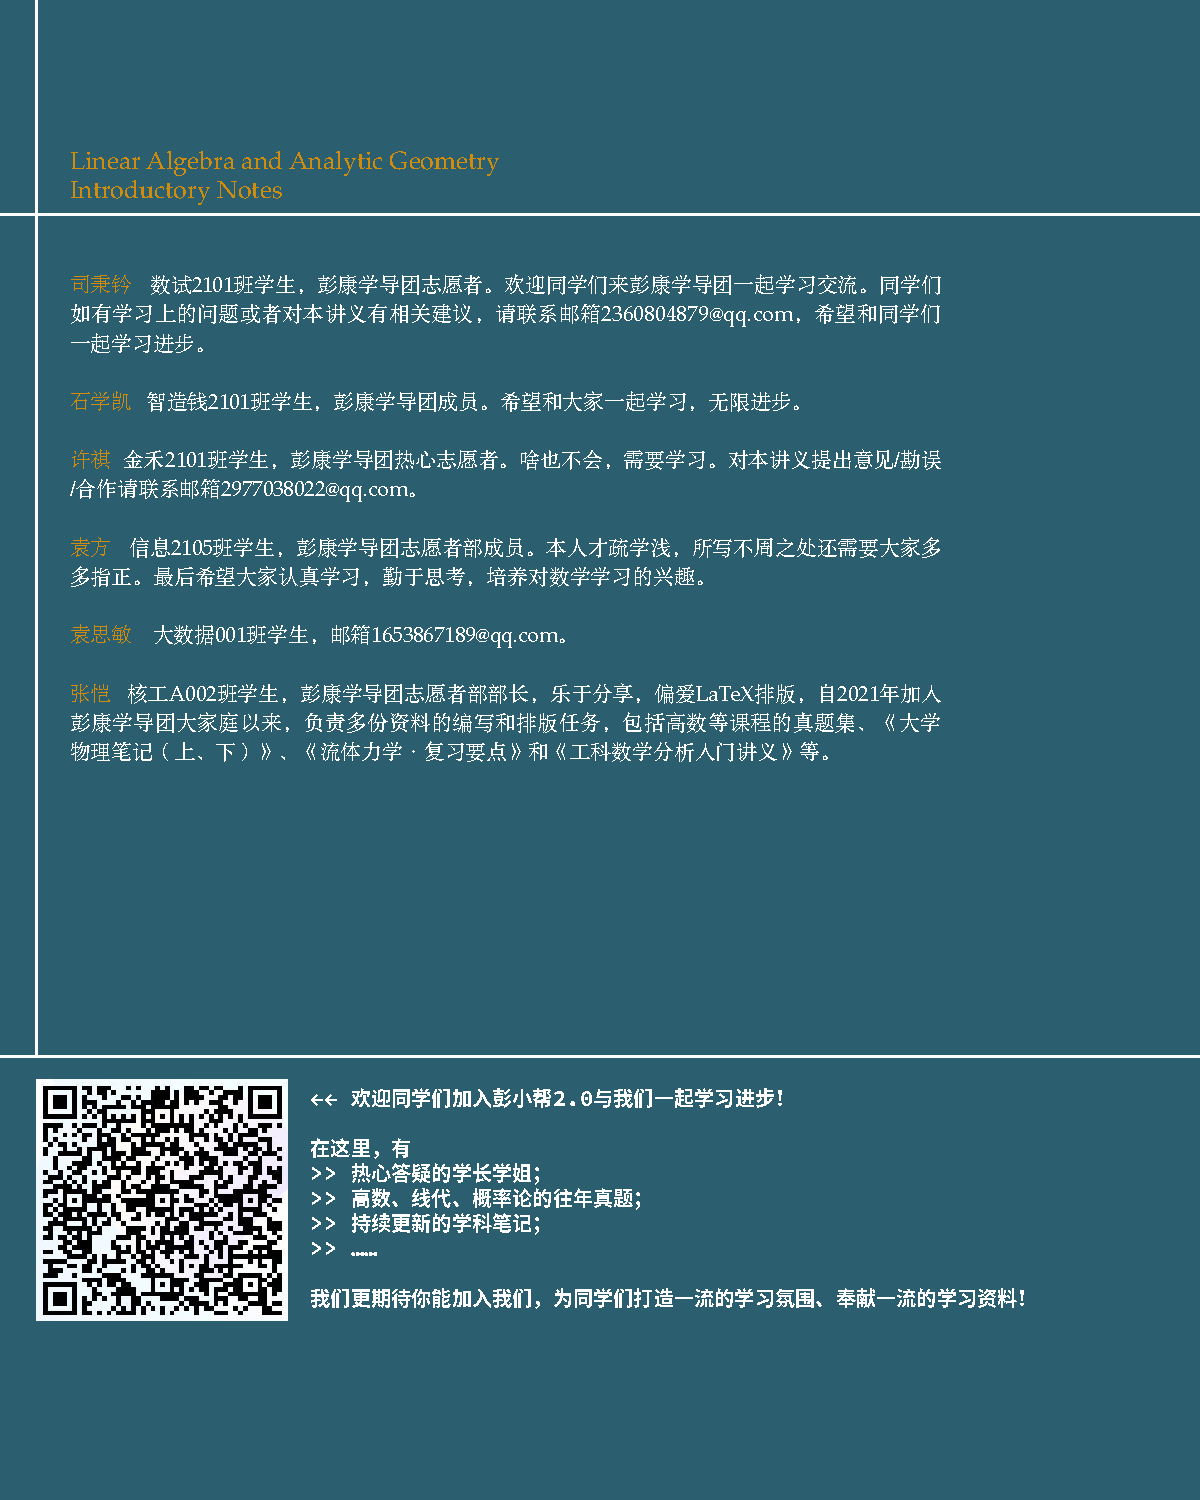
\includepdf[noautoscale=true, width=\paperwidth]{backcover.pdf}
\end{document}
